\documentclass[10pt,a4paper]{beamer}
\usepackage[utf8]{inputenc}
\usepackage[T1]{fontenc}
\usepackage[english]{babel}
% \usepackage{hyperref}
\usepackage{amssymb,amsthm,amsmath,amsfonts}
\usepackage{lmodern}
% \usepackage{units}
% \usepackage{hyperref}
\usepackage{tikz}
% \usepackage{tikzsymbols}
\usetikzlibrary{calc}
\usetikzlibrary{fixedpointarithmetic}
\usepackage{fp}
\usepackage{graphicx}
% \bibliographystyle{plain}
\usepackage{epsfig}
\usepackage{epstopdf}
% \usepackage{makeidx}
% \usepackage{gloss}
\usepackage{algorithmic}
% \usepackage{algorithm}
\usepackage{todonotes}

% \usepackage{xkeyval} 

\def\glossname{Glossaire}
%\bibliographystyle{alpha} % plain-fr si rapport en français

% \usepackage[usenames,dvipsnames]{pstricks}
% \usepackage{epsfig}
% \usepackage{pst-grad} % For gradients}}
% \usepackage{pst-plot}



\theoremstyle{plain}
\newtheorem{thm}{Theorem}[part]
\theoremstyle{definition} 
\newtheorem{lem}[thm]{Lemma}
\theoremstyle{definition} 
\newtheorem{cor}[thm]{Corollary}
\theoremstyle{definition} 
\newtheorem{prop}[thm]{Proposition}
\theoremstyle{definition} 
\newtheorem{defi}[thm]{Definition}
\theoremstyle{remark} 
\newtheorem{rem}[thm]{Remark}
\theoremstyle{remark} 
\newtheorem{exe}[thm]{Example}

\useoutertheme{split}
\useinnertheme{rounded}
\usecolortheme{whale}
\usecolortheme{orchid}
\usecolortheme[named=blue]{structure}
\makeatletter

\setbeamertemplate{headline}{%
%  \begin{beamercolorbox}[wd=\paperwidth,ht=3pt]{logo in head}%
%    This is cut by Uni-KL projector
%  \end{beamercolorbox}
  \leavevmode \@tempdimb=2.4375ex%
  \ifnum\beamer@subsectionmax<\beamer@sectionmax%
    \multiply\@tempdimb by\beamer@sectionmax%
  \else%
    \multiply\@tempdimb by\beamer@subsectionmax%
  \fi%
  \ifdim\@tempdimb>0pt%
    \advance\@tempdimb by 1.825ex%
    \begin{beamercolorbox}[wd=.5\paperwidth,ht=\@tempdimb]{section in head/foot}%
      \vbox to\@tempdimb{\vfil\insertsectionnavigation{.5\paperwidth}\vfil}%
    \end{beamercolorbox}%
    \begin{beamercolorbox}[wd=.5\paperwidth,ht=\@tempdimb]{logo in head}%
    \vbox to\@tempdimb{\vfil \hbox to .5\paperwidth{\hfil
  
\includegraphics[height=8mm]{Images/uvsq-logo-cmjn.jpg}\hskip 8mm}\vfil}%
    \end{beamercolorbox}%
  \fi%
}
\setbeamertemplate{footline}{%
  \leavevmode%
  \hbox{\begin{beamercolorbox}[wd=.5\paperwidth,ht=2.5ex,dp=1.125ex,leftskip=.3cm plus1fill,rightskip=.3cm]{author in head/foot}%
    \usebeamerfont{author in head/foot}\insertshortauthor
  \end{beamercolorbox}%
  \begin{beamercolorbox}[wd=.5\paperwidth,ht=2.5ex,dp=1.125ex,leftskip=.3cm,rightskip=.3cm plus1fil]{title in head/foot}%
    \usebeamerfont{title in head/foot}\insertshorttitle \hfill
    \insertframenumber/\inserttotalframenumber
  \end{beamercolorbox}}%
  \vskip0pt%
}
\makeatother
\definecolor{uvsqvert}{RGB}{91,172,41}
\definecolor{uvsqbleu}{RGB}{15,152,209}
% \setbeamercolor{section in head/foot}{fg=black,bg=uvsqvert}
% \setbeamercolor{subsection in head/foot}{fg=black,bg=uvsqvert!80}
\setbeamercolor{logo in head}{fg=black,bg=white}
% \def\insertsubsectionnavigation#1{\hbox to #1{%
%   \hfill 
\includegraphics[height=8mm]{Images/uvsq-logo-cmjn.jpg}}}
\definecolor{pacificcream}{cmyk}{.05,.05,.15,0}


\setbeamerfont{block title}{size={}}
\beamertemplatenavigationsymbolsempty

\newcommand{\orangebox}[2]{
\setbeamercolor{uppercol}{fg=white,bg=orange}
\setbeamercolor{lowercol}{fg=black,bg=pacificcream}

\begin{beamerboxesrounded}[upper=uppercol,lower=lowercol,shadow=true]{
#1 }  #2
\end{beamerboxesrounded} }

\newcommand{\bluebox}[2]{
\setbeamercolor{upperblue}{fg=white,bg=blue}
\setbeamercolor{lowercol}{fg=black,bg=pacificcream}

\begin{beamerboxesrounded}[upper=upperblue,lower=lowercol,shadow=true]{
#1 }  #2
\end{beamerboxesrounded} }

\newenvironment{orangeitemize}{\setbeamertemplate{itemize item}{$\bullet$}\begin{itemize}}{\end{itemize}}
\newenvironment{grassgreenitemize}{\setbeamertemplate{itemize item}{\textcolor{grassgreen}{$\bullet$}} \begin{itemize}}{\end{itemize}}
\newenvironment{blackitemize}{\setbeamertemplate{itemize item}{\textcolor{black}{$\bullet$}} \begin{itemize}}{\end{itemize}}


% \logo{
\includegraphics[height=8mm]{Images/uvsq-logo-cmjn.jpg}} 
% \addtobeamertemplate{footline}{\hfill\insertframenumber/ \inserttotalframenumber \hspace{2em}\null}

\def\algorithmicrequire{\textbf{Input:}}
\def\algorithmicensure{\textbf{Output:}}

%\DeclareMathOperator{\ker}{ker}

\def\red#1{\textcolor{red}{#1}}
\def\blu#1{\textcolor{blue}{#1}}

\tikzset{position/.style args={#1:#2 from #3}{%
  at=(#3.#1),anchor=#1+180,shift=(#1:#2)}}%
\tikzstyle{lambda}=[very thick,draw=blue,->]
\tikzstyle{mu}=[very thick,draw=red,->]

\begin{document}

\author{
Cyril Hugounenq
}
%\title[Structure of $\ell$-isogeny volcanoes applied to Couveignes' algorithm]{Structure of $\ell$-isogeny volcanoes applied to Couveignes' algorithm}
\title[Volcans et calculs d'isogénies]{
Volcans et calculs d'isogénies}
\institute{Université de Versailles Saint-Quentin-en-Yvelines}
\date{25 Septembre, 2017}


\begin{frame}
\titlepage

\hfill

\includegraphics[scale=0.1]{Images/digiteo.jpg}\hfill

\includegraphics[height=10mm]{Images/uvsq-logo-cmjn.jpg}
\end{frame}
%\maketitle
%faire un plan
%faire un rappel sur les courbes elliptiques
\begin{frame}
\frametitle{Summary}
\tableofcontents
\end{frame}

%%%%%%%%%%%%%%%%%%%%%%%%%%%%%%%%%%%%%%%%%%%%%%%%%%%%%%%%%%%%
%%%%%%%%%%%%%%%%%%%%%%%%%%%%%%%%%%%%%%%%%%%%%%%%%%%%%%%%%%%%
\section{Reminder on isogenies}
%parler aussi de la cryptographie sur les courbes elliptiques

\begin{frame}
\frametitle{Points defined on an elliptic curve}

\begin{defi}[Courbe Elliptique]
Soit $\mathbb{K}$ un corps de caractéristique différente de $2$ et $3$, une courbe elliptique $E$ peut être définie à l'aide d'une équation de Weierstrass: 
%la variété projective associée à l'équation
\begin{equation*}
\label{eq:weierstrass-proj}
E:=\{ (X,Y) \in \overline{\mathbb{K}} , Y^2=X^3+a_4X+a_6 \} \cup O_E
\end{equation*}
avec $a_4,a_6$ des éléments de $\overline{\mathbb{K}}$. $O_E$ est appelé le \emph{point à l'infini}. 
%Dès lors que $a_4,a_6$ appartiennent à $\mathbb{K}$ alors la courbe est dite
%définie sur $\mathbb{K}$.
\end{defi}
%Partir directement en coordonnées projectives .
%Faire un dessin de courbe elliptique

\begin{figure}
\begin{center}

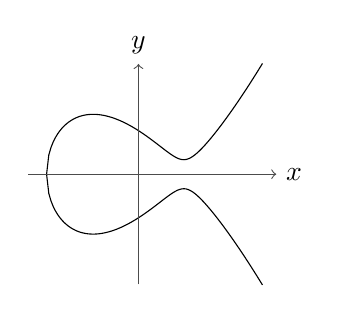
\begin{tikzpicture}[scale=0.35,domain=-10/3:4.5,samples=100,yscale=1/2]
          \begin{scope}[fixed point arithmetic]
            
            \draw plot (\x,{sqrt(\x*\x*\x+(3-100/9)*\x+10)});
            \draw plot (\x,{-sqrt(\x*\x*\x+(3-100/9)*\x+10)});
			\draw[->,color=black!70!white] (-4,0) -- (5,0);
			\draw (5,0) node[right] {$x$};
			\draw [->,color=black!70!white] (0,-8) -- (0,8);
			\draw (0,8) node[above] {$y$};
          \end{scope}
\end{tikzpicture}
\end{center}
%\caption{Représentation d'une courbe elliptique}
\end{figure}
\end{frame}
%%%%%%%%%%%%%%%%%%%%%%%%%%%%%%%%%%%%%%%%%%%%%%%%%%%%%%%%%%%%%
\begin{frame}
\frametitle{Loi de Groupe sur une courbe elliptique}


\begin{figure}
\begin{center}

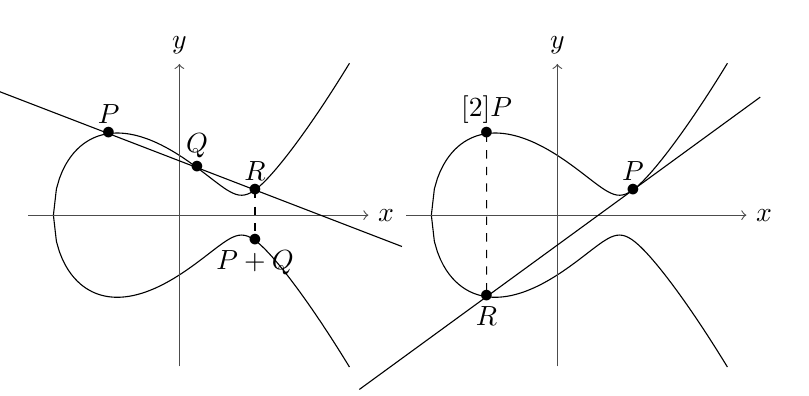
\begin{tikzpicture}[scale=0.480,domain=-10/3:4.5,samples=100,yscale=1/2]
          \begin{scope}[fixed point arithmetic]
            \begin{scope}[fixed point arithmetic]
              \coordinate (Q) at (2, -4/3) {};
              \coordinate (-Q) at (2, 4/3) {};
              \coordinate (-2Q) at (-1079/576, 59653/13824);
              \coordinate (3Q) at (2319138/4977361, 27920423524/11104492391);
            \end{scope}

            \draw plot (\x,{sqrt(\x*\x*\x+(3-100/9)*\x+10)});
            \draw plot (\x,{-sqrt(\x*\x*\x+(3-100/9)*\x+10)});
			\draw[->,color=black!70!white] (-4,0) -- (5,0);
			\draw (5,0) node[right] {$x$};
			\draw [->,color=black!70!white] (0,-8) -- (0,8);
			\draw (0,8) node[above] {$y$};			
			
            \draw[shorten >=-2cm, shorten <=-2cm] (-2Q) -- (-Q);
            \draw[dashed] (-Q) -- (Q);

%            \begin{scope}[/dot/.style={draw,circle,inner sep=1pt,fill},
%              every label/.style={inner sep=5pt,font=\scriptsize}]
%              \draw (-2Q) node[/dot,label=$P$] {}
%               (3Q) node[/dot,label=$Q$] (G) {}
%              (-Q) node[/dot,label=$R$] {};
%              \draw[label position=right,label distance=5pt] (Q) node[/dot,label=$P+Q$] {};
%            \end{scope}
            \draw (-2Q) node{$\bullet$};
            \draw (-2Q) node[above]{$P$};
            \draw (3Q) node{$\bullet$};
            \draw (3Q) node[above]{$Q$};
            \draw (-Q) node{$\bullet$};
            \draw (-Q) node[above]{$R$};
            \draw (Q) node{$\bullet$};
            \draw (Q) node[below]{$P+Q$};
          \end{scope}

          \begin{scope}[xshift=10cm,fixed point arithmetic]
            \draw plot (\x,{sqrt(\x*\x*\x+(3-100/9)*\x+10)});
            \draw plot (\x,{-sqrt(\x*\x*\x+(3-100/9)*\x+10)});
			\draw[->,color=black!70!white] (-4,0) -- (5,0);
			\draw (5,0) node[right] {$x$};
			\draw [->,color=black!70!white] (0,-8) -- (0,8);
			\draw (0,8) node[above] {$y$};		
		
            \begin{scope}[fixed point arithmetic]
              \coordinate (-Q) at (2, 4/3) {};
              \coordinate (-2Q) at (-1079/576, 59653/13824);
              \path let \p1 = (-2Q) in coordinate (2Q) at (\x1,-\y1);
            \end{scope}

            \draw[shorten >=-2cm, shorten <=-2cm] (-Q) -- (2Q);
            \draw[dashed] (-2Q) -- (2Q);

%            \begin{scope}[/dot/.style={draw,circle,inner sep=1pt,fill},
%              every label/.style={inner sep=5pt,font=\scriptsize}]
%              \draw (-Q) node[/dot] {$P$}
%              (-2Q) node[/dot] (G) {$[2]P$};
%              \draw[label position=below] (2Q) node[/dot] {$R$};
%            \end{scope}
            
            \draw (-Q) node{$\bullet$};
            \draw (-Q) node[above]{$P$};
            \draw (-2Q) node{$\bullet$};
            \draw (-2Q) node[above]{$[2]P$};
            \draw (2Q) node{$\bullet$};
            \draw (2Q) node[below]{$R$};
%			 \begin{scope}[/dot/.style={draw,circle,inner sep=1pt,fill},
%              every label/.style={inner sep=5pt,font=\scriptsize}]
%              \draw (-2Q) node[/dot,label=$P$] {}
%               (3Q) node[/dot,label=$Q$] (G) {}
%              (-Q) node[/dot,label=$R$] {};
%              \draw[label position=right,label distance=5pt] (Q) node[/dot,label=$P+Q$] {};
%            \end{scope}
%          \end{scope}            
            
          \end{scope}
        \end{tikzpicture}

\end{center}
\end{figure}

\pause

\begin{prop}[Silverman, '86]
L'ensemble des points d'une courbe elliptique forme un groupe abélien pour la loi additive.
\end{prop}


\end{frame}

%%%%%%%%%%%%%%%%%%%%%%%%%%%%%%%%%%%%%%%%%%%%%%%%%%%%%%%%%%%%%

\begin{frame}
\bluebox{Multiplication scalaire}{On définit alors pour une courbe elliptique 
$E$ et un entier $n$:
\begin{align*}
[n] \;:\; E & \to E\\
P & \mapsto [n] P
\end{align*}}
\pause 
\hfill
\bluebox{Problème du logarithme discret sur une courbe elliptique $E$}
{
\begin{algorithmic}[1]
\REQUIRE $P \in E$ le générateur du groupe $G:=\langle P \rangle$, $Q=[x]P \in G$;
\ENSURE $x$.
\end{algorithmic}
}
%Il manque un lien avec la suite..
%Dire que c'est donc intéressant de se pencher sur des applications qui permettent de conserver cette propriété....
\end{frame}


%%%%%%%%%%%%%%%%%%%%%%%%%%%%%%%%%%%%%%%%%%%%%%%%%%%%%%%%%%%%%
%%%%%%%%%%%%%%%%%%%%%%%%%%%%%%%%%%%%%%%%%%%%%%%%%%%%%%%%%%%%%


\begin{frame}
\frametitle{Refresher on isogenies}
\bluebox{Isogenies}{
\begin{itemize}
\item $E$ and $E'$ two elliptic curves, an isogeny is  a surjective morphism $\phi: E \rightarrow E'$ such that $\phi(0_{E})=0_{E'}$. Isogenies are
\begin{itemize}
 \item group morphisms (with finite kernel),
 \item algebraic maps (of finite degree).
\end{itemize}
 
\item  If the isogeny has degree $\ell$, we call it an \emph{$\ell$-isogeny},

\item We say that $E$ and $E'$ are \emph{$\ell$-isogenous} if there exist an $\ell$-isogeny between them.

\item In this talk: only \emph{rational} isogenies (i.e.\ Galois-equivariant maps).

%\item We say that $E$ and $E'$ are isogenous if there exist an isogeny $\phi$ between the two curves.

%\item Moreover if the isogeny $\phi$ is $\textbf{separable}$ then we have $\deg \phi = | \ker(\phi) |$ and if $\ell= \deg \phi $ then we say that the curves $E$ and $E'$ are $\ell$-isogenous.
\end{itemize}
}
\pause

% \begin{thm} 
% Let $G\subset E$ be a subgroup of points of order $\ell$. There is an isogeny $\phi:E\to E'$ of degree $\ell$ such that $\ker\phi = G$.
% \end{thm}

% For \emph{separable} isogenies, this defines a bijection between isogenies and finite subgroups.

\textbf{Example:}
Let $\ell$ be an integer, the \emph{scalar multiplication map}
\begin{align*}
[\ell] \;:\; E &\to E\\
P &\mapsto [\ell] P
\end{align*}
is an isogeny of degree $\ell^2$.

\end{frame}

%%%%%%%%%%%%%%%%%%%%%%%%%%%%%%%%%%%%%%%%%%%%%%%%%%%%%%%%%%%%

\begin{frame}
\frametitle{Explicit isogenies}

\bluebox{Explicit isogenies}{
Separable isogenies of degree $\ell$ are represented by rational maps in Weierestrass form
%\[
%\left( x ,y \right) \mapsto \left( \frac{n(x)=45x^9+67x^7+57x^6+97x^5+7+100x^2+78x+67}{d(x)(x^4+51x^2+67x+61)^2}, y\left(\frac{n(x)}{d(x)\right)^'} \right)
%\]
\vspace{-1mm}
\[
\left( x,y \right) \mapsto \left(\frac{n(x)}{d(x)}, cy \left( \frac{n(x)}{d(x)} \right)' \right)
\]
with $n(x)$ a polynomial of degree $\ell$ and $d(x)$ a polynomial of degree $\ell-1$.


}

%\begin{exe} 
%$E$ an elliptic curve defined over $\mathbb{F}_q$, then we define an $\ell$-isogeny by a point: $P$ of order $\ell$
%\[ \phi: E \rightarrow E/ \left\langle P \right\rangle \]
%\end{exe}

\bluebox{V\'elu's formulas}{
From the knowledge of its kernel we can explicitly write down the isogeny:
\begin{itemize}
    \item Let $G=\ker\phi$, then $\displaystyle d(X)=\prod_{P \in G\setminus\{0_E\}}(X-x(P))$;
    \item V\'elu's formulas: from $d(X)$ we deduce $n(X)/d(X)$;
    %\item Complexity quasi-linear in $\ell = \#G$.
\end{itemize}
}

\end{frame}

%%%%%%%%%%%%%%%%%%%%%%%%%%%%%%%%%%%%%%%%%%%%%%%%%%%%%%%%%%%%

\begin{frame}
\frametitle{Motivation}
%We focus on one specific subproblem in the Schoof-Elkies-Atkin point counting  algorithm:
%\medskip
\bluebox{Explicit isogeny computation problem}
{
 Let $\mathbb{F}_q$ be a finite field of characteristic $p$. 
 Given $E$, $E'$   two $r$-isogenous elliptic curves defined over $\mathbb{F}_q$,
 compute an $r$-isogeny $\phi:E\to E'$.
}
\medskip

%\bluebox{Disclaimer:}{This is \textbf{not} the dominant step in SEA.}

Applications:
\begin{itemize}
\item Schoof-Elkies-Atkin point counting algorithm,
\item ECC cryptanalysis: [Gaudry,~Hess,~Smart '02],
\item Hash functions: [Charles,~Goren,~Lauter '07],
\item Trapdoors: [Teske~'06],
\item Post quantum cryptography: [Rotostev,~Stolbunov~'06], [De~Feo,~Jao,~Pl\^ut~'11].
\end{itemize}

\end{frame}

%%%%%%%%%%%%%%%%%%%%%%%%%%%%%%%%%%%%%%%%%%%%%%%%%%%%%%%%%%%%

\begin{frame}
\frametitle{Previous work}

Let $p$ be the characteristic of $\mathbb{F}_q$.

\begin{itemize}
\item{} [Elkies~'92/'98],  %[Charlap, Colay, Robbins '91], 
[Bostan,~Morain,~Salvy,~Schost~'08] use $\tilde{O}(r)$ operations in $\mathbb{F}_q$, work only for $r < 2p$. Specific to the SEA case.
\item{} [Couveignes~'94] any characteristic, $\tilde{O}(r^3
p^{O(1)})$ operations.
\item{} [Lercier~'97] only $p=2$.
\item{} [Couveignes~'96], [De Feo~'10] any characteristic, $\tilde{O}(r^2
p^{O(1)})$ operations.
\item{} [Lercier,~Sirvent~'08], [Lairez,~Vaccon~'16] works for every $p$ using $\tilde{O}(r)$ operations in $\mathbb{F}_q$. Specific to the SEA case.
\end{itemize}
\begin{itemize}

%\item[$\rightarrow$] we focus on the medium characteristic case ($n\gg p/\log(p)$),

\item[$\rightarrow$] We want to modify Couveignes' algorithm to obtain an algorithm with complexity $\tilde{O}(r^2)$ but with no exponential dependency in $\log(p)$.

\end{itemize}
\end{frame}

%%%%%%%%%%%%%%%%%%%%%%%%%%%%%%%%%%%%%%%%%%%%%%%%%%%%%%%%%%%%
%%%%%%%%%%%%%%%%%%%%%%%%%%%%%%%%%%%%%%%%%%%%%%%%%%%%%%%%%%%%

\section{Couveignes' algorithm}

\begin{frame}
\frametitle{Torsion points of elliptic curves}

\vspace{-1mm}

\bluebox{Torsion points}{
Let $E$ be an elliptic curve defined over a finite field $\mathbb{F}_q$, and let $m>0$
\vspace{-1.5mm}
\[E[m]= \{ P \in E(\bar{\mathbb{F}}_q) , [m]P=0_E \} \]

For \emph{ordinary} elliptic curves
\vspace{-1.5mm}
\begin{align*}
E[\ell^k]&\simeq\mathbb{Z}/\ell^k\mathbb{Z} \times \mathbb{Z}/\ell^k\mathbb{Z} \quad \textit{with } \ell \neq p \\
E[p^k]&\simeq\mathbb{Z}/p^k\mathbb{Z}
\end{align*}
}
\pause
\bluebox{Couveignes' algorithm (compute an $r$-isogeny $\phi:E\to E'$)}{
Compute $\phi$ by interpolation over $E[p^k]$:
\begin{itemize}
\item Compute generators $P,P'$ of $E[p^k],E'[p^k]$;
\item Interpolate $\phi$, assuming it maps $[u]P\mapsto [u]P'$ for all $u \in \mathbb{Z}/p^k\mathbb{Z}$;
\item Test whether $\phi$ is an isogeny.\\
    In case it is not, replace $P'$ with a multiple $[a]P'$ and start again.
\end{itemize}

}
\end{frame}

%%%%%%%%%%%%%%%%%%%%%%%%%%%%%%%%%%%%%%%%%%%%%%%%%%%%%%%%%%%%

\begin{frame}
\frametitle{Couveignes algorithm (1996)}
\bluebox{}{ %\cite{DBLP:conf/ants/Couveignes96}}{
\begin{algorithmic}[1]
\REQUIRE $E, E'$ two $r$-isogenous curves on $\mathbb{F}_{p^n}$ 
\ENSURE $\phi: E \rightarrow E'$ of degree $r$
\end{algorithmic}}

\begin{enumerate}
\item Select the least $k$ such that $p^k >  4r$;
\item Compute generators $P$ of
  $E[p^k]$ and $P'$ of $E'[p^k]$;
\item Compute $T=\prod(X-x([u]P))$ with $1\le u \le \frac{p^k-1}{2}$;
\item For each $a \in \left( \mathbb{Z}/p^k\mathbb{Z}\right)^{\times}$:\hfill $O(r)$
 \begin{enumerate}
  \item Compute the interpolation polynomial
    $L$ such that
    $L (x ([u] P)) = x([a\, u\,]P' )$ for all
    $u \in \mathbb{Z}/p^k \mathbb{Z}$;
    \hfill $\tilde{O}(r p^{O(1)})$
  \item Use a  rational reconstruction  algorithm 
    to compute a rational
    fraction $F=L\bmod{T}$ of degrees~$(r, r-1)$;
    \hfill $\tilde{O}(r)$
  \item If $F$ defines an isogeny of degree $r$, return it and
    stop.
  \end{enumerate}
\end{enumerate}
%Complexity polynomial in $p$. 
\pause
\bluebox{Goal} {Replace $E[p^k]$ by \boldmath $E[\ell^k]$ \unboldmath for
a small prime $\ell \neq p$.}
\end{frame}

%%%%%%%%%%%%%%%%%%%%%%%%%%%%%%%%%%%%%%%%%%%%%%%%%%%%%%%%%%%%

\begin{frame}

\frametitle{An $\ell$-adic Couveignes' algorithm?}
\bluebox{}{
Our goal is to work with \boldmath $E[\ell^k]\simeq \left(\mathbb{Z}/\ell^k \mathbb{Z} \right)^2$ \unboldmath 
%Our goal is to work with \textcolor{red}{$E[\ell^k]= \left(\mathbb{Z}/\ell^k \mathbb{Z} \right)^2$}  
instead of $E[p^k]$ to remove the polynomial dependency in $p$.
\begin{itemize}

%\item[$\Rightarrow$] main drawback: $E[\ell^{\frac{k}{2}}]=\left(\mathbb{Z}/\ell^{\frac{k}{2}} \mathbb{Z} \right)^2$ thus for two basis $\langle P,Q \rangle=E[\ell^{\frac{k}{2}}]$, $\langle P',Q' \rangle=E'[\ell^{\frac{k}{2}}]$ we have to test $O(\ell^{\frac{4k}{2}})=O(r^2)$ mapping candidates before finding the good one for the interpolation.
\item $E[p^k] = \langle P\rangle\simeq\left(\mathbb{Z}/p^{k} \mathbb{Z}
\right)$ \hfill with $p^{k} \approx r$
\item $E[\ell^k] = \langle P,Q\rangle\simeq\left(\mathbb{Z}/\ell^{k}
\mathbb{Z} \right) \times \left(\mathbb{Z}/\ell^{k} \mathbb{Z} \right)$
\hfill with $\color{red} \ell^{2k} \approx r$
\end{itemize}}
\pause
\begin{columns}
\begin{column}{0.48\textwidth}

\bluebox{$p$-adic}{
Let $P\in E\quad$ and $\quad P'\in E'$
\[
P \mapsto [a] P'  \qquad a\in(\mathbb{Z}/p^k\mathbb{Z})^*
\]

$\Rightarrow O(r)$ possibilities.
}
\end{column}
\begin{column}{0.55\textwidth}
\bluebox{$\ell$-adic}{
Let $P,Q \in E\quad$ and $\quad P',Q' \in E'$
\begin{gather*}
\begin{pmatrix}
P\\Q
\end{pmatrix}
\mapsto
\begin{pmatrix}
a & b \\
c & d
\end{pmatrix}
\begin{pmatrix}
P'\\Q'
\end{pmatrix}
\\[1ex]
\text{with $\left(\begin{smallmatrix}a&b\\c&d\end{smallmatrix}\right)\in \mathsf{GL}_2(\mathbb{Z}/\ell^k\mathbb{Z})$ invertible}.
\end{gather*}
$\Rightarrow O(r^2)$ possibilities.
}
\end{column}
\end{columns}

%\pause
%\begin{center}
%    Ouch! Can we restrict the choices for $\left(\begin{smallmatrix}a&b\\c&d\end{smallmatrix}\right)$?
%\end{center}

\end{frame}

%%%%%%%%%%%%%%%%%%%%%%%%%%%%%%%%%%%%%%%%%%%%%%%%%%%%%%%%%%%%
%%%%%%%%%%%%%%%%%%%%%%%%%%%%%%%%%%%%%%%%%%%%%%%%%%%%%%%%%%%%
%\section{An $\ell$-adic Couveignes algorithm (special case)}
\section{An $\ell$-adic Couveignes algorithm (special case)}

\begin{frame}
\frametitle{Frobenius vs isogenies}
\begin{defi}[Frobenius Endomorphism]
$E$ an ordinary elliptic curve defined over $\mathbb{F}_q$. The function
\[ \pi:(x,y) \mapsto (x^q,y^q)\] is called Frobenius endomorphism. It
satisfies a quadratic equation \[ \pi^2 - t_\pi \pi + q = 0.\]
\end{defi}

We are only working with rational isogenies $\psi:E \to E'$, i.e.
\[
\pi_{E'} \circ \psi =\psi \circ \pi_{E}.
 \]


\end{frame}

%%%%%%%%%%%%%%%%%%%%%%%%%%%%%%%%%%%%%%%%%%%%%%%%%%%%%%%%%%%%


%\begin{frame}
%    \begin{columns}
%        \begin{column}{0.8\textwidth}
%            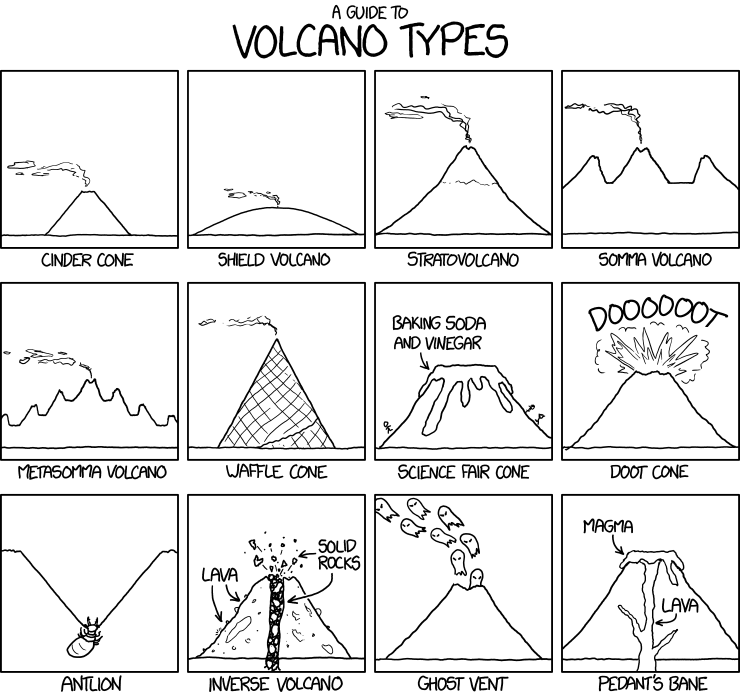
\includegraphics[height=\textheight]{Images/xkcd.png}
%        \end{column}
%        \begin{column}{0.2\textwidth}
%            \href{http://xkcd.com/1714/}{xkcd.com/1714}
%        \end{column}
%    \end{columns}
%\end{frame}

%%%%%%%%%%%%%%%%%%%%%%%%%%%%%%%%%%%%%%%%%%%%%%%%%%%%%%%%%%%%


\begin{frame}
\vspace{-4mm}
  \begin{center}
    \begin{tabular}{p{13em}p{2em}p{13em}}
Subgroup of size $\ell$  & $\Leftrightarrow$ &     $\ell$-isogeny \pause \\[2mm]
      
    Subgroup of size $\ell$ stable by $\pi$   & $\Leftrightarrow$ & Rational $\ell$-isogeny 
    \end{tabular}
  \end{center}


\pause
Assume that $\pi$ splits modulo $\ell$:
i.e. its minimal polynomial factors as
\[ (\pi-\red \lambda)(\pi- \blu \mu ) \quad \text{with} \quad \red \lambda \neq \blu \mu \bmod \ell \]


\pause
\begin{center}
  \begin{tabular}{p{13em}p{2em}p{13em}}
     \raggedright Two eigenspaces in $E[\ell]$
     \mbox{$\ker(\pi-\red \lambda), \ker( \pi- \blu \mu)$}
     & $\Rightarrow$  
     & \raggedright Two rational $\ell$-isogenies
    \mbox{of direction $\red \lambda, \blu \mu $}
  \end{tabular}
\end{center}
%
\bluebox{Isogeny graph}{
\begin{figure}[h]
	\begin{center}
	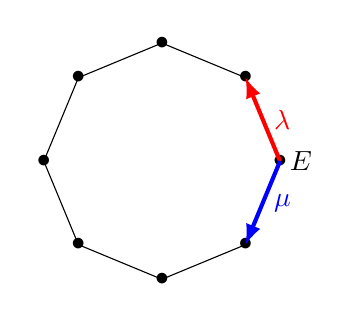
\begin{tikzpicture}[scale=0.3]
	\coordinate (A) at (0:5);
	\coordinate (B) at (45:5);
	\coordinate (C) at (90:5);
	\coordinate (D) at (135:5);
	\coordinate (E) at (180:5);
	\coordinate (F) at (225:5);
	\coordinate (G) at (270:5);
	\coordinate (H) at (315:5);
	\draw (A)--(B)--(C)--(D)--(E)--(F)--(G)--(H)--(A);	
		
	\draw (A) node[right]{$E$};
	\draw (A) node{$\bullet$};
	\draw (B) node{$\bullet$};
	\draw (C) node{$\bullet$};
	\draw (D) node{$\bullet$};
	\draw (E) node{$\bullet$};
	\draw (F) node{$\bullet$};
	\draw (G) node{$\bullet$};
	\draw (H) node{$\bullet$};
	
	\draw[line width=1.5pt,red,-latex] (A)--(B) node[midway,right]{$\color{red} \lambda$};
	\draw[line width=1.5pt,blue,-latex] (A)--(H) node[midway,right]{$\color{blue} \mu$};
		\end{tikzpicture}	
	\end{center}
\end{figure}
}

\end{frame}


%%%%%%%%%%%%%%%%%%%%%%%%%%%%%%%%%%%%%%%%%%%%%%%%%%%%%%%%%%%%

\begin{frame}
  \bluebox{Fact}{
    Let $\phi$ be an $r$-isogeny with $\ell \nmid r$, then $\phi$ preserves the kernels of the $\ell$-isogenies of \emph{direction} $\red \lambda, \blu \mu $.}

  To interpolate $\phi$ over $E[\ell^k]$, we want to compute two cyclic
  $\ell^k$-subgroups of direction $\red \lambda, \blu \mu $. 

  \begin{figure}[h]
    \begin{center}
      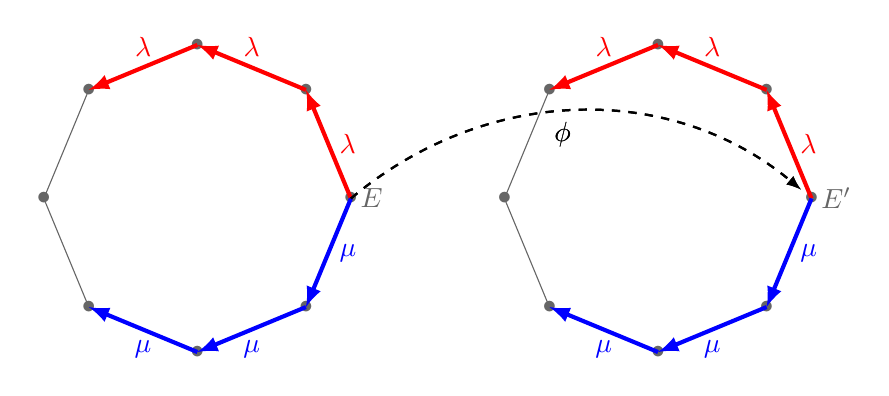
\begin{tikzpicture}[scale=0.39]
        \foreach \s/\e in {0/E,15cm/E'} {
          \begin{scope}[xshift=\s,black!60]
            \coordinate (A) at (0:5);
            \coordinate (B) at (45:5);
            \coordinate (C) at (90:5);
            \coordinate (D) at (135:5);
            \coordinate (E) at (180:5);
            \coordinate (F) at (225:5);
            \coordinate (G) at (270:5);
            \coordinate (H) at (315:5);

            \draw (A) node{$\bullet$};
            \draw (A) node[right]{$\e$};
            \draw (B) node{$\bullet$};
            \draw (C) node{$\bullet$};
            \draw (D) node{$\bullet$};
            \draw (E) node{$\bullet$};
            \draw (F) node{$\bullet$};
            \draw (G) node{$\bullet$};
            \draw (H) node{$\bullet$};

            \draw (A)--(B)--(C)--(D)--(E)--(F)--(G)--(H)--(A);		
            \begin{scope}[-latex]
              \draw[line width=1.5pt,red] (A)--(B) node[midway,right]{$\color{red} \lambda$};
              \draw[line width=1.5pt,blue] (A)--(H) node[midway,right]{$\color{blue} \mu$};
              \uncover<2->{
                \draw[line width=1.5pt,red] (B)--(C) node[midway,above]{$\color{red} \lambda$};
                \draw[line width=1.5pt,blue] (H)--(G) node[midway,below]{$\color{blue} \mu$};
              }
              \uncover<3->{
                \draw[line width=1.5pt,red] (C)--(D) node[midway,above]{$\color{red} \lambda$};
                \draw[line width=1.5pt,blue] (G)--(F) node[midway,below]{$\color{blue} \mu$};
              }
            \end{scope}
          \end{scope}

          \draw[dashed,thick,-latex,shorten >=5pt] (0:5) to[bend left=40] node[below left] {$\phi$} (0:20);
        }
      \end{tikzpicture}	
    \end{center}
  \end{figure}

  \begin{uncoverenv}<3->
    \begin{itemize}
    \item We call $\red{E[\ell^k]_\lambda}\oplus\blu{E[\ell^k]_\mu}$ a
      \emph{horizontal} decomposition;
    \item SEA literature calls this an \emph{isogeny cycle} [Couveignes, Morain '94].
    \end{itemize}
  \end{uncoverenv}

\end{frame}

%%%%%%%%%%%%%%%%%%%%%%%%%%%%%%%%%%%%%%%%%%%%%%%%%%%%%%%%%%%%

\begin{frame}

\bluebox{Towards an $\ell$-adic Couveignes' algorithm ($\pi$ splits modulo $\ell$)}{
\begin{algorithmic}[1]
\REQUIRE $E, E'$ two $r$-isogenous curves on $\mathbb{F}_{q}$ 
\ENSURE $\phi: E \rightarrow E'$ of degree $r$
\end{algorithmic}}

\bluebox{}{\textbf{Fact:} $\phi$ maps 
$\color{red}{E[\ell^k]_{{\lambda}}} \color{black}{\rightarrow} \color{red}{E'[\ell^k]_{{\lambda}}}$  
and 
$\color{blue}{E[\ell^k]_{{\mu}}} \color{black}{\rightarrow} \color{blue}{E'[\ell^k]_{{\mu}}}$.
 }

\begin{enumerate}
\item Select the least $k$ such that  $\ell^{2k}>4r$.
\medskip
\item Compute $\langle \red P , \blu Q \rangle = \color{red}{E[\ell^k]_{{\lambda}}} \color{black} \oplus \color{blue}{E[\ell^k]_{{\mu}}} $\\
 and $\langle \color{red} P' \color{black}, \color{blue} Q'\color{black} \rangle = \color{red}{E'[\ell^k]_{{\lambda}}} \color{black} \oplus \color{blue}{E'[\ell^k]_{{\mu}}} $
%\item Deduce $\to$ $\langle{\color{red}P},{\color{blue}Q}\rangle=E[\ell^k]$ and $\langle{\color{red}P'},{\color{blue}Q'}\rangle=E'[\ell^k]$;
\medskip
\item For each \textbf{invertible diagonal} matrix
  $\left ( \begin{smallmatrix}a & 0\\ 0 & b
\end{smallmatrix}\right )$ in $(\mathbb{Z}/\ell^k \mathbb{Z})^{2 \times 2}$:
\hfill\only<2>{$O(r)$}
  \begin{enumerate}

  \item Compute the interpolation polynomial
    $L$ sending\\
    $\color{red}P\mapsto [a]P'$ and $\color{blue}Q\mapsto [b]Q'$;
\hfill\only<2>{$\tilde{O}(r \ell^{O(1)})$}
	\item Use a  rational reconstruction  algorithm 
    to compute a rational
    fraction $F$ of degrees~$(r, r-1)$;
\hfill\only<2>{$\tilde{O}(r)$}
  \item If $F$ defines an isogeny of degree $r$, return it and
    stop.
  \end{enumerate}
\end{enumerate}
\end{frame}

%%%%%%%%%%%%%%%%%%%%%%%%%%%%%%%%%%%%%%%%%%%%%%%%%%%%%%%%%%%%
%%%%%%%%%%%%%%%%%%%%%%%%%%%%%%%%%%%%%%%%%%%%%%%%%%%%%%%%%%%%
%\section{An $\ell$-adic Couveignes algorithm}

\begin{frame}
\frametitle{The general case}

Denote by $\mathcal{O}$ (resp. $\mathcal{O}'$) the endomorphism ring of $E$ (resp. $E'$)
\vspace{-4mm}
\begin{columns}
\begin{column}{6cm}
%\includegraphics[scale=.66]{Images/ordres-l.eps}
\begin{figure}
\begin{center}

\begin{tikzpicture}[scale=0.55]
\coordinate (A) at (0,1.5);
\coordinate (AB) at (1,1.5);
%\coordinate (AZ) at (-1.5,1.5);	
\coordinate (B) at (0,5);
\coordinate (BB) at (1,5);
%\coordinate (BZ) at (-1.5,5.2);
%\coordinate (BZ2) at (-1.5,4.8);
\coordinate (C) at (0,10);
\coordinate (CB) at (1,10);
%\coordinate (CZ) at (-1.5,10);
\draw (A) node[left]{$\mathbb{Z} + \ell^2 \mathcal{O}$} node{$\bullet$};
\draw (B) node[left]{$\mathbb{Z} + \ell \mathcal{O}$} node{$\bullet$};
\draw (C) node[left]{$\mathcal{O}$} node{$\bullet$};
\draw (A)--(B)node[midway,left] {$\ell$};
\draw (B)--(C) node[midway,left] {$\ell$};
%\draw (CZ)--(BZ)[dashed]  node[midway,left] {$\ell$};
%\draw (BZ2)--(AZ)[dashed]  node[midway,left] {$\ell$};
\begin{scope}[yshift=10cm]
	\begin{scope}[xshift=4.3cm]
		\node (A) at (-3,0) {$\bullet$};
		\node (B) at (3,0) {$\bullet$};
		\node (C) at (270:1.2) {$\bullet$};
		\node (D) at (90:1.5) {};
		%\draw[-] (A.center) to[bend right=25] (C.center);
		\draw[-,dashed] (A.center) to[bend left=40] (B.center);
		%\draw[-] (B.center) to[bend left=25] (C.center);
		%\draw[-,dashed] (B.center) to[bend right] (D.center);
		\only<1-2>{
		\draw[-] (A.center) to[bend right=40] (B.center);
		}
		\only<3-3>{
		\draw[-] (C.center) to[bend right=20] (B.center);
		\draw[line width=1.5pt,red,->] (A.center) to[bend right=20] (C.center);
		}
			\begin{scope}[xshift=-3cm]
			\coordinate (A) at (0,0);
			\coordinate (C) at (270:4.2);
			\coordinate (CA) at (265:7.5);
			\coordinate (CB) at (275:7.5);
			\draw (C)--(CA);
			\draw (C)--(CB);
			\draw (CA) node{$\bullet$};
			\draw (CB) node{$\bullet$};
			\draw (A) node{$\bullet$};
			\draw (C) node{$\bullet$};
			\draw (A)--(C);
			\end{scope}
			\begin{scope}[xshift=3cm]
			\coordinate (A) at (0,0);
			\coordinate (C) at (270:4.2);
			\coordinate (CA) at (265:7.5);
			\coordinate (CB) at (275:7.5);
			\draw (C)--(CA);
			\draw (C)--(CB);
			\draw (CA) node{$\bullet$};
			\draw (CB) node{$\bullet$};
			\draw (A) node{$\bullet$};
			\draw (C) node{$\bullet$};
			\draw (A)--(C);
			\end{scope}
			\begin{scope}[yshift=-1.2cm]
			\coordinate (A) at (0,0);
			\coordinate (C) at (270:4.2);
			\coordinate (CA) at (265:7.5);
			\coordinate (CB) at (275:7.5);
			\draw (C)--(CA);
			\draw (C)--(CB);
			\draw (CA) node{$\bullet$};
			\draw (CB) node{$\bullet$};
			\draw (A) node{$\bullet$};
			\draw (C) node{$\bullet$};
			\draw (A)--(C);
            \only<1-1>{
            \draw[line width=1.5pt,red,->] (A)--(C);
            }
            \only<2-2>{
			\draw[line width=1.5pt,red,<-] (A)--(C);            
            }
			\end{scope}
	\end{scope}
\end{scope}

%faire des fleches courbees avec les indices \ell et \ell^2


\end{tikzpicture}
\end{center}		
\end{figure}

\end{column}
\begin{column}{4cm}

\begin{lem}[Kohel 1996]
$E$ and $E'$ two elliptic curves defined over $\mathbb{F}_q$, $\psi :E \rightarrow E'$ an $\ell$-isogeny. Then we say that $\psi$ is
\begin{enumerate}
\item  \textbf<1>{descending} if $\ell=[\mathcal{O} : \mathcal{O}']$
\item \textbf<2>{ascending} if $\ell=[\mathcal{O}':\mathcal{O}]$,
\item \textbf<3>{horizontal} if $\mathcal{O}=\mathcal{O}'$.
\end{enumerate}
\end{lem}
%\begin{defi}
%The index $f=[\mathcal{O}_K : \mathcal{O}]$ is called the conductor of $\mathcal{O}$.
%\end{defi}
\end{column}

\end{columns}
\end{frame}


%%%%%%%%%%%%%%%%%%%%%%%%%%%%%%%%%%%%%%%%%%%%%%%%%%%%%%%%%%%%

\begin{frame}
\frametitle{A guide to volcano types}
\begin{figure}[h]
		\begin{center}
        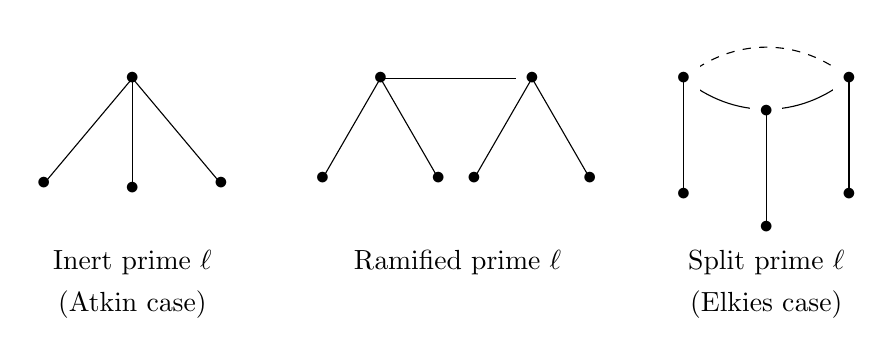
\begin{tikzpicture}[scale=0.35]
        \coordinate (A) at (0,0);
		\coordinate (B) at (230:5);
		\coordinate (C) at (270:4);
		\coordinate (D) at (310:5);
		\draw (A) node{$\bullet$};
		\draw (B) node[fill=white]{$\bullet$};
		\draw (C) node[fill=white]{$\bullet$};
		\draw (D) node[fill=white]{$\bullet$};
		\node at (0,-6.7) {Inert prime $\ell$};
		\node at (0,-8.2) {(Atkin case)};
		\draw (A)--(B);
		\draw (A)--(C);
		\draw (A)--(D);		
		\begin{scope}[xshift=9cm]
		\coordinate (A) at (0,0);
		\coordinate (B) at (5.5,0);
		\coordinate (C) at (240:4.2);
		\coordinate (D) at (300:4.2);
		\draw (A) node[fill=white]{$\bullet$};
		\draw (B) node[fill=white]{$\bullet$};
		\draw (C) node[fill=white]{$\bullet$};
		\draw (D) node[fill=white]{$\bullet$};
		\node at (2.8,-6.7) {Ramified prime $\ell$};
		\draw (A)--(B);
		\draw (A)--(C);
		\draw (A)--(D);
		\end{scope}
		
		\begin{scope}[xshift=14.5cm]
		\coordinate (A) at (0,0);
		\coordinate (C) at (240:4.2);
		\coordinate (D) at (300:4.2);
		\draw (A) node[fill=white]{$\bullet$};
		\draw (C) node[fill=white]{$\bullet$};
		\draw (D) node[fill=white]{$\bullet$};
		\draw (A)--(C);
		\draw (A)--(D);
		\end{scope}
		
		\begin{scope}[xshift=23cm]
		\node (A) at (-3,0) {$\bullet$};
		\node (B) at (3,0) {$\bullet$};
		\node (C) at (270:1.2) {$\bullet$};
		\node (D) at (90:1.5) {};
		\node at (0,-6.7) {Split prime $\ell$};
		\node at (0,-8.2) {(Elkies case)};
		%\draw[-] (A.center) to[bend right=25] (C.center);
		\draw[-,dashed] (A.center) to[bend left=40] (B.center);
		%\draw[-] (B.center) to[bend left=25] (C.center);
		%\draw[-,dashed] (B.center) to[bend right] (D.center);
		\draw[-] (A.center) to[bend right=40] (B.center);
			\begin{scope}[xshift=-3cm]
			\coordinate (A) at (0,0);
			\coordinate (C) at (270:4.2);
			\draw (A) node[fill=white]{$\bullet$};
			\draw (C) node[fill=white]{$\bullet$};
			\draw (A)--(C);
			\end{scope}
			\begin{scope}[xshift=3cm]
			\coordinate (A) at (0,0);
			\coordinate (C) at (270:4.2);
			\draw (A) node[fill=white]{$\bullet$};
			\draw (C) node[fill=white]{$\bullet$};
			\draw (A)--(C);
			\end{scope}
			\begin{scope}[yshift=-1.2cm]
			\coordinate (A) at (0,0);
			\coordinate (C) at (270:4.2);
			\draw (A) node[fill=white]{$\bullet$};
			\draw (C) node[fill=white]{$\bullet$};
			\draw (A)--(C);
			\end{scope}
		\end{scope}
		\end{tikzpicture}
		%\end{center}
		\caption{The three shapes of volcanoes of $2$-isogenies }
		
		\end{center} 
		\end{figure}
In the rest of this talk we consider first volcanoes with cyclic crater (Elkies case), then volcanoes with one point on the crater (Atkin case).
%\begin{figure}[hbtp]
%\centering
%\includegraphics[scale=0.4]{Images/duo-volcan-wo-label.png}
%\caption{Volcano with one point on the crater, and two points}
%\end{figure}
\end{frame}

%%%%%%%%%%%%%%%%%%%%%%%%%%%%%%%%%%%%%%%%%%%%%%%%%%%%%%%%%%%%
\begin{frame}

\bluebox{Elkies prime}{We say that $\ell$ is an \emph{Elkies prime} if the characteristic polynomial of $\pi$ factors over $\mathbb{Z}_{\ell}$ as
\[
\pi^2 - t_{\pi}\pi + q = (\pi - \red \lambda) (\pi - \blu \mu), \quad \textsf{with } \red \lambda \neq \blu \mu,
\]
where $h=v_{\ell}(\red \lambda - \blu \mu)$ can be $\geqslant 1$.
}
Since for any $P \in  E[\ell^h]$ we have:
\[
\pi(P)= [\red \lambda ] P = [\blu \mu ] P
\]
we cannot immediately distinguish kernels of isogenies with direction $\red
\lambda$ from those with direction $\blu \mu$.

\medskip
Thus in Couveignes' algorithm  we have to work with $E[\ell^{k}]$ with $k \geqslant h+1$ to be able to determine $P \in \red{ E[\ell^{h+1}]_{ \lambda}}$ such that: 
%Thus we have to work with $E[\ell^{h+1}]$ to get $P \in \red{ E[\ell^{h+1}]_{ \lambda}}$ such that:
\[
\pi(P)= [\red \lambda ] P \neq [\blu \mu ] P
\]
We must therefore now assume that $k \geqslant h+1$.

\end{frame}


%
%\begin{frame}
%%Diapo sur le Frobenius....
%%We want to study the action of the Frobenius on the $\ell$ torsion:
%The Frobenius endomorphism acts on $E[\ell^k]$ as a $2\times2$ invertible matrix:
%\[
%\pi|E[\ell^k]:
%\begin{pmatrix}
%a & b \\
%c & d 
%\end{pmatrix} \bmod{\ell^k}
%\]
%%%%%%%%%%%%%%%%%%%%%%%%%%%%%%%%%%%%%%%%%%%%%%%%%%%%%%%%%%%%


\begin{frame}

\begin{prop}[De Feo, H., Pl\^ut, Schost]\label{prop:matrice-Frobenius}
%Let $E$ be a curve on a crater of an $\ell$-isogeny volcano.
%Then there exists a unique $a \in \{ 0,\ell, \dots, \ell^{h-1}  \}$
%such that $\pi|T_\ell(E)$~is conjugate, over~$\mathbb{Z}_\ell$,
%to the matrix $\left ( \begin{smallmatrix}\lambda & a\\ 0 & \mu
%\end{smallmatrix}\right )$.
% where $a ∈ ℤ$, $0 ≤ a ≤ ℓ^{h} - 1$,
In the Elkies case the action of the Frobenius endomorphism $\pi$ on $E[\ell^{h+1}]$~is conjugate, over~$\mathbb{Z}_{\ell}$,
to a unique matrix \[\left ( \begin{matrix}{\color{red}\lambda} & a\\ 0 &
{\color{blue}\mu} \end{matrix}\right ), \]  with $a \in \{ 1,\ell, \dots,
\ell^{h-1}, 0  \}$, and $a = 0$ iff~$E$ lies on the crater.

%Moreover $a = 0$ if~$E$ lies on the crater.
%and else $h - v_{\ell}(a)$~is the depth of~$E$ in the volcano.
\end{prop}

\begin{figure}
\begin{center}

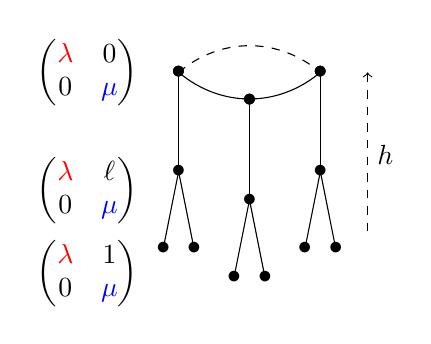
\begin{tikzpicture}[scale=0.30]
\coordinate (A) at (0,1.5);
\coordinate (AB) at (1,1.5);
\coordinate (AZ) at (-1.5,1.5);	
\coordinate (B) at (0,5);
\coordinate (BB) at (1,5);
\coordinate (BZ) at (-1.5,5.2);
\coordinate (BZ2) at (-1.5,4.8);
\coordinate (C) at (0,10);
\coordinate (CB) at (1,10);
\coordinate (CZ) at (-1.5,10);
\draw (A) node[left]{$\left( \begin{matrix}
\color{red}{\lambda} & 1 \\
0 & \color{blue}{\mu}
\end{matrix} \right) \color{black} $}; %node{$\bullet$};
\draw (B) node[left]{$ \left( \begin{matrix}
\color{red}{\lambda} & \ell \\
0 & \color{blue}{\mu}
\end{matrix} \right) \color{black} $}; %node{$\bullet$};
\draw (C) node[left]{$ \left( \begin{matrix}
\color{red}{\lambda} & 0 \\
0 & \color{blue}{\mu}
\end{matrix} \right) \color{black} $}; %node{$\bullet$};
%\draw (A)--(B);
%\draw (B)--(C);
%\draw (CZ)--(BZ)[dashed]  node[midway,left] {$\ell$};
%\draw (BZ2)--(AZ)[dashed]  node[midway,left] {$\ell$};
\begin{scope}[yshift=10cm]
	\begin{scope}[xshift=4.3cm]
		\node (A) at (-3,0) {$  \bullet $};
		\node (B) at (3,0) {$   \bullet$};
		\node (C) at (270:1.2) {$ \bullet \color{black}$};
		\node (D) at (90:1.5) {};
		%\draw[-] (A.center) to[bend right=25] (C.center);
		\draw[-,dashed] (A.center) to[bend left=40] (B.center);
		%\draw[-] (B.center) to[bend left=25] (C.center);
		%\draw[-,dashed] (B.center) to[bend right] (D.center);
		\draw[-] (A.center) to[bend right=40] (B.center);
		\draw (A) node{$  \bullet $};
		\draw (B) node{$  \bullet $};
		\draw (C) node{$  \bullet $};
		%\draw[line width=2.5pt,red,->] (A.center) to[bend right=20] (C.center);
			\begin{scope}[xshift=-3cm]
			\coordinate (A) at (0,0);
			\coordinate (C) at (270:4.2);
			\coordinate (CA) at (265:7.5);
			\coordinate (CB) at (275:7.5);
			\draw (C)--(CA);
			\draw (C)--(CB);
			\draw (A)--(C);
			\draw (CA) node{$ \bullet$};
			\draw (CB) node{$\bullet$};
			\draw (A) node{$  \bullet \color{black}$};
			\draw (C) node{$  \bullet \color{black}$};
			\end{scope}
			\begin{scope}[xshift=3cm]
			\coordinate (A) at (0,0);
			\coordinate (C) at (270:4.2);
			\coordinate (CA) at (265:7.5);
			\coordinate (CB) at (275:7.5);
			\draw (C)--(CA);
			\draw (C)--(CB);
			\draw (A)--(C);
			\draw (CA) node{$ \bullet$};
			\draw (CB) node{$\bullet$};
			\draw (A) node{$ \bullet$};
			\draw (C) node{$ \bullet$};
			\end{scope}
			\begin{scope}[yshift=-1.2cm]
			\coordinate (A) at (0,0);
			\coordinate (C) at (270:4.2);
			\coordinate (CA) at (265:7.5);
			\coordinate (CB) at (275:7.5);
			\draw (C)--(CA);
			\draw (C)--(CB);
			\draw (A)--(C);
			\draw (CA) node{$ \bullet$};
			\draw (CB) node{$ \bullet$};
			%\draw (A) node{$\bullet$};
			\draw (C) node{$ \bullet$};
			\draw (A) node{$ \bullet$};
			
			
			%(C) node[left]{$\mathcal{O}$} node{$\bullet$};			
			
			\end{scope}
			\coordinate (F) at (5,0);
			\coordinate (G) at (5,-7);
			\draw[dashed,<-] (F)--(G) node[midway,right]{$h$};
	\end{scope}
\end{scope}

%faire des fleches courbees avec les indices \ell et \ell^2

\end{tikzpicture}
\end{center}
\end{figure}
\end{frame}

%%%%%%%%%%%%%%%%%%%%%%%%%%%%%%%%%%%%%%%%%%%%%%%%%%%%%%%%%%%%


\begin{frame}
%Does it work the same with general volcanoes of $\ell$-isogenies?
%\pause
We assume that $E$ lies on the crater (we can reduce to this case easily).
 
%Let $P \in E[\ell^{h+1}]$ such that  $\pi(P)=\red \lambda(P)$
%We compute $\ell^k$-isogenies of kernel $\ker(\pi-\blu \mu)$.
\begin{columns}
\begin{column}{5cm}
\bluebox{Volcano with height $h=0$}{
\begin{figure}[h]
	\begin{center}
	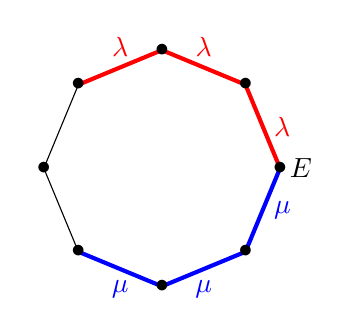
\begin{tikzpicture}[scale=0.3]
	\coordinate (A) at (0:5);
	\coordinate (B) at (45:5);
	\coordinate (C) at (90:5);
	\coordinate (D) at (135:5);
	\coordinate (E) at (180:5);
	\coordinate (F) at (225:5);
	\coordinate (G) at (270:5);
	\coordinate (H) at (315:5);
	\draw (A)--(B)--(C)--(D)--(E)--(F)--(G)--(H)--(A);		
	\draw[line width=1.5pt,red] (A)--(B) node[midway,right]{$\color{red} \lambda$};
	\draw[line width=1.5pt,blue] (A)--(H) node[midway,right]{$\color{blue} \mu$};
	\draw[line width=1.5pt,red] (B)--(C) node[midway,above]{$\color{red} \lambda$};
	\draw[line width=1.5pt,blue] (H)--(G) node[midway,below]{$\color{blue} \mu$};
	\draw[line width=1.5pt,red] (C)--(D) node[midway,above]{$\color{red} \lambda$};
	\draw[line width=1.5pt,blue] (G)--(F) node[midway,below]{$\color{blue} \mu$};
		
	\draw (A) node[right]{$E$};
	\draw (A) node{$\bullet$};
	\draw (B) node{$\bullet$};
	\draw (C) node{$\bullet$};
	\draw (D) node{$\bullet$};
	\draw (E) node{$\bullet$};
	\draw (F) node{$\bullet$};
	\draw (G) node{$\bullet$};
	\draw (H) node{$\bullet$};
	\end{tikzpicture}	
	\end{center}
\end{figure}
}
$\ker(\pi- \blu \mu\; | \; E[\ell^k])$ is a cyclic group of size $\ell^k$.
\end{column}
\begin{column}{5.5cm}
\bluebox{Volcano with height $h=2$}{\begin{center}
\tikzstyle{lambda1}=[lambda,draw=blue!60!green]
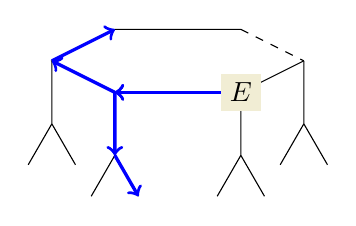
\begin{tikzpicture}[scale=0.40]
% \coordinate (A) at (0,-1.2);
% \coordinate (B) at (-3,0);
% \coordinate (C) at (-1.2,.7);
% \coordinate (D) at (1.2,.7);
% \coordinate (E) at (3,0);
\coordinate (A) at (2,-1);
\coordinate (B) at (-2,-1);
\coordinate (C) at (-4,0);
\coordinate (D) at (-2,1);
\coordinate (E) at (2,1);
\coordinate (F) at (4,0);
\draw (F)--(A)--(B)--(C)--(D)--(E); \draw[dashed] (E)--(F);

\coordinate[position=-90:.8 from A] (AA);
\coordinate[position=-60:.6 from AA] (AA0);
\coordinate[position=-120:.6 from AA] (AA1);
\draw (A)--(AA)--(AA0); \draw (AA)--(AA1);
\coordinate[position=-90:.8 from B] (BB);
\coordinate[position=-60:.6 from BB] (BB0);
\coordinate[position=-120:.6 from BB] (BB1);
\draw (B)--(BB)--(BB0); \draw (BB)--(BB1);
\coordinate[position=-90:.8 from C] (CC);
\coordinate[position=-60:.6 from CC] (CC0);
\coordinate[position=-120:.6 from CC] (CC1);
\draw (C)--(CC)--(CC0); \draw (CC)--(CC1);
\coordinate[position=-90:.8 from F] (FF);
\coordinate[position=-60:.6 from FF] (FF0);
\coordinate[position=-120:.6 from FF] (FF1);
\draw (F)--(FF)--(FF0); \draw (FF)--(FF1);
\draw<2>[lambda] (A)--(B); \draw<2>[lambda] (B)--(BB);
\draw<2>[lambda] (BB)--(BB0);
\draw<3>[lambda] (A)--(B); \draw<3>[lambda] (B)--(C);
\draw<3>[lambda] (C)--(D);
\node[fill=pacificcream] at (A) {$E$};
\end{tikzpicture}
\end{center}
}
\textbf{Problem:} if $h \geqslant 1$
then $\ker(\pi- \blu \mu  \;| \; E[\ell^k])
\simeq (\mathbb Z/\ell^k) \!\times\! (\mathbb Z/\ell^h)$ is not cyclic,
and contains $\ell^h$ cyclic subgroups of order $\ell^k$.

\end{column}
\end{columns}

\end{frame}


%%%%%%%%%%%%%%%%%%%%%%%%%%%%%%%%%%%%%%%%%%%%%%%%%%%%%%%%%%%%

%\begin{frame}
%Our aim is to compute an horizontal decomposition: $E[\ell^k]_{\lambda} \oplus E[\ell^k]_{\mu}$ of $E[\ell^k]$ (aka isogeny cycle in the SEA litterature).

%We will proceed step by step since with diagonalisation of $\ker (\pi -\lambda), \ker (\pi -\mu)  \bmod \ell^{h+1}$ we get an horizontal decomposition $E[\ell^k]_{\lambda} \oplus E[\ell^k]_{\mu}$.


%\end{frame}

%%%%%%%%%%%%%%%%%%%%%%%%%%%%%%%%%%%%%%%%%%%%%%%%%%%%%%%%%%%%


\begin{frame}
\frametitle{Walking on the crater}
\bluebox{Fact}{
    Let $\phi$ be an $r$-isogeny with $\ell \nmid r$, then $\phi$ preserves the kernels of the horizontal $\ell^k$-isogenies of direction $\red \lambda, \blu \mu $.}
%\textbf{Goal:} compute the kernel of horizontal $\ell^k$-isogenies (codomain curves lying on the crater).


We proceed step by step by walking along the crater according to the direction $ \blu \mu$. %to compute the kernels of the horizontal $\ell^3$-isogeny of direction $\blu \mu $.
\begin{center}
\begin{tikzpicture}[scale=0.37]
\begin{scope}[yshift=10cm]
	\begin{scope}[xshift=4.3cm]
		\node (A) at (-3,0) {$\bullet$};
		\node (B) at (3,0) {$\bullet$};
		\node (C) at (270:1.2) {$\bullet$};
		\node (D) at (125:1.2) {$E_2$};
		%\draw[-] (A.center) to[bend right=25] (C.center);
		\draw[-] (D.center) to[bend right=20] (A.center);
		\only<1-2>{		
		\draw[-] (D.center) to[bend left=18] (B.center);
		}
		\only<3->{
		\draw[line width=1.5pt,blue,->] (D.center) to[bend left=20] (B.center);
		
		\node (F) at (1.25,1.30) {$\color{blue} \mu$};
		%\node (F2) at (1.25,0.50) {$\color{blue} \psi_2$};		
		}
		\only<5->{
		\draw[line width=1.5pt,blue,->] (D.center) to[bend right=20] (A.center);		
		}
		\only<5->{		
		\node (F2) at (-2.25,1) {$\color{blue} \mu$};
		}
%		\only<4->{
%		\draw[line width=1.5pt,red,->] (D.center) to[bend left=20] (B.center);
%		\draw[-] (D.center) to[bend right=20] (A.center);
%		\node (F) at (1.25,1.30) {$\color{red} \lambda$};		
%		}
		%\draw[-] (B.center) to[bend left=25] (C.center);
		%\draw[-,dashed] (B.center) to[bend right] (D.center);
		\only<1->{
		\draw[line width=1.5pt,blue,->] (C.center) to[bend right=20] (B.center); 
		\node (F) at (1.5,-0.5) {$\color{blue} \mu$};	
		%\node (F2) at (1.5,-1.5) {$\color{blue} \psi$};	
		}
%		\only<2->{
%		\draw[line width=1.5pt,red,<-] (C.center) to[bend right=20] (B.center); 
%		\node (F) at (1.5,-0.5) {$\color{red} \lambda$};		
%		}
		
			\begin{scope}[xshift=-3cm]
			\coordinate (A) at (0,0);
			\coordinate (C) at (270:4.2);
			\coordinate (CA) at (265:7.5);
			\coordinate (CB) at (275:7.5);
			\draw (C)--(CA);
			\only<1>{
			\draw (C)--(CB);}
			\only<2->{
			\draw (C)--(CB);}
			\only<1-3>{			
			\draw (A)--(C);}
			\only<4->{
			\draw (A)--(C);}
			\only<5>{
			\draw [line width=1.5pt,blue] (C)--(A);
			\draw [line width=1.5pt,blue] (C)--(CA);
			}
			%just to have a 6th slide
			\only<6>{
			\draw (C)--(A);
			\draw (C)--(CA);
			}
%			\draw (A) node[fill=white]{$30$};
%			\draw (C) node[fill=white]{$98$};
%			\draw (CA) node[fill=white]{$22$};
%			\draw (CB) node[fill=white]{$74$};
			\draw (A) node[fill=white]{$E_3$};
			\draw (C) node[fill=white]{$\bullet$};
			\draw (CA) node[fill=white]{$\bullet$};
			\draw (CB) node[fill=white]{$\bullet$};
			\end{scope}
			\begin{scope}[xshift=3cm]
			\coordinate (A) at (0,0);
			\coordinate (C) at (270:4.2);
			\coordinate (CA) at (265:7.5);
			\coordinate (CB) at (275:7.5);
			\draw (C)--(CA);
			\draw (C)--(CB);
			\draw (A)--(C);
			\only<1>{
			\draw [line width=1.5pt,blue] (C)--(CB);
			\draw [line width=1.5pt,blue] (A)--(C);
			}
%			\draw (A) node[fill=white]{$65$};
%			\draw (C) node[fill=white]{$60$};
%			\draw (CA) node[fill=white]{$39$};
%			\draw (CB) node[fill=white]{$62$};
			\draw (A) node[fill=white]{$E_1$};
			\only<2-3>{\draw (A) node[fill=yellow!50!white,shape=circle]{$E_1$};}
			\draw (C) node[fill=white]{$\bullet$};
			\draw (CA) node[fill=white]{$\bullet$};
			\draw (CB) node[fill=white]{$\bullet$};
			\end{scope}
			\begin{scope}[yshift=-1.2cm]
			\coordinate (A) at (0,0);
			\coordinate (C) at (270:4.2);
			\coordinate (CA) at (265:7.5);
			\coordinate (CB) at (275:7.5);
			\draw (C)--(CA);
			\draw (C)--(CB);
			\draw (A)--(C);
			\draw (A) node[fill=white]{$E$};
			\only<1>{\draw (A) node[fill=yellow!50!white,shape=circle]{$E$};}
			\draw (C) node[fill=white]{$\bullet$};
			\draw (CA) node[fill=white]{$\bullet$};
			\draw (CB) node[fill=white]{$\bullet$};
%			\draw (CA) node[fill=white]{$45$};
%			\draw (CB) node[fill=white]{$68$};
			\end{scope}
			\begin{scope}[shift={(D)}]
			\coordinate (A) at (0,0);
			\coordinate (C) at (270:4.2);
			\coordinate (CA) at (265:7.5);
			\coordinate (CB) at (275:7.5);
			\draw [dashed] (C)--(CA);
			\draw [dashed] (C)--(CB);
			\draw [dashed] (A)--(C);
			\draw (C) node[color=black!90]{$\bullet$};
			\draw (CA) node[color=black!90]{$\bullet$};
			\draw (CB) node[color=black!90]{$\bullet$};
			\only<3>{
			\draw [line width=1.5pt,blue] (C)--(A);
			\draw [line width=1.5pt,blue] (C)--(CA);
			}
			\only<1-3,5->{\draw (A) node[fill=white]{$E_2$};}			
			\only<4>{\draw (A) node[fill=yellow!50!white,shape=circle]{$E_2$};}
			\end{scope}
	\coordinate (A) at (-3,0);
	\coordinate (C) at (270:1.2);
	\only<1->{
	\draw (A.center) to[bend right=20] (C.center);
	}
	\draw (A) node[fill=white]{$E_3$};
	\only<1>{
	\draw (C) node[fill=yellow!50!white,shape=circle]{$E$};
	}	
	\only<2->{
	\draw (C) node[fill=white]{$E$};
	}
	\end{scope}
\end{scope}

\end{tikzpicture}
\end{center}
\end{frame}

%%%%%%%%%%%%%%%%%%%%%%%%%%%%%%%%%%%%%%%%%%%%%%%%%%%%%%%%%

\begin{frame}

\bluebox{Towards an $\ell$-adic Couveignes' algorithm ($\ell$ an Elkies prime)}{
\begin{algorithmic}[1]
\REQUIRE $E, E'$ two $r$-isogenous curves on $\mathbb{F}_{q}$ 
\ENSURE $\phi: E \rightarrow E'$ of degree $r$
\end{algorithmic}}

\bluebox{}{\textbf{Fact:} $\phi$ maps 
$\color{red}{E[\ell^k]_{{\lambda}}} \color{black}{\rightarrow} \color{red}{E'[\ell^k]_{{\lambda}}}$  
and 
$\color{blue}{E[\ell^k]_{{\mu}}} \color{black}{\rightarrow} \color{blue}{E'[\ell^k]_{{\mu}}}$.
 }

\begin{enumerate}
\item Select the least $k$ such that  $\ell^{2k}>4r$.
\medskip
\item Compute $\langle \red P , \blu Q \rangle = \color{red}{E[\ell^k]_{{\lambda}}} \color{black} \oplus \color{blue}{E[\ell^k]_{{\mu}}} $\\
 and $\langle \color{red} P' \color{black}, \color{blue} Q'\color{black} \rangle = \color{red}{E'[\ell^k]_{{\lambda}}} \color{black} \oplus \color{blue}{E'[\ell^k]_{{\mu}}} $ generators of horizontal $\ell^k$-isogenies of directions $\color{red} \lambda \color{black}, \color{blue} \mu$.  
%\item Deduce $\to$ $\langle{\color{red}P},{\color{blue}Q}\rangle=E[\ell^k]$ and $\langle{\color{red}P'},{\color{blue}Q'}\rangle=E'[\ell^k]$; Rajouter le coût de cela...
\medskip
\item For each \textbf{invertible diagonal} matrix
  $\left ( \begin{smallmatrix}a & 0\\ 0 & b
\end{smallmatrix}\right )$ in $(\mathbb{Z}/\ell^k \mathbb{Z})^{2 \times 2}$:
\hfill\only<2>{$O(r)$}
  \begin{enumerate}

  \item Compute the interpolation polynomial
    $L$ sending\\
    $\color{red}P\mapsto [a]P'$ and $\color{blue}Q\mapsto [b]Q'$;
\hfill\only<2>{$\tilde{O}(r \ell^{O(1)})$}
	\item Use a  rational reconstruction  algorithm 
    to compute a rational
    fraction $F$ of degrees~$(r, r-1)$;
\hfill\only<2>{$\tilde{O}(r)$}
  \item If $F$ defines an isogeny of degree $r$, return it and
    stop.
  \end{enumerate}
\end{enumerate}
\end{frame}

%%%%%%%%%%%%%%%%%%%%%%%%%%%%%%%%%%%%%%%%%%%%%%%%%%%%%%%%%%%%

\begin{frame}
\frametitle{Limitations of the Elkies case}
 \bluebox{Finding an Elkies prime $\ell$}{
  \begin{itemize}
  \item The complexity depends polynomially on the auxiliary prime $\ell$.
  \item Ideally we would like to work with $\ell=2$.
  \item In practice half of all $\ell$ are expected to be Elkies primes.
  \item In theory we can only prove $\ell \leq O(\log(q))$ for almost
    all $q$ and curves $E,E'$ (see [Shparlinski,~Sutherland~'14]).
\end{itemize}
  }
\end{frame}

%%%%%%%%%%%%%%%%%%%%%%%%%%%%%%%%%%%%%%%%%%%%%%%%%%%%%%%%%%%% 

\begin{frame}
%\section{Atkin Case}
\section{An $\ell$-adic Couveignes algorithm}
\frametitle{Atkin case}
\bluebox{Atkin prime}{We say that $\ell$ is an \emph{Atkin prime} if the characteristic polynomial of $\pi$: 
\[
\pi^2 - t_{\pi}\pi + q 
\]
is irreducible over $\mathbb{Z}_{\ell}$}
%Thus we are not able to distinguish two different eigenspaces, 
Thus the method used with \emph{Elkies prime} using two different eigenspaces cannot be applied. 
\begin{figure}
\begin{center}
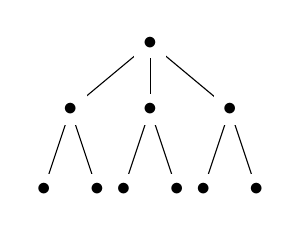
\begin{tikzpicture}[scale=0.225]
\begin{scope}[yshift=10.5cm,xshift=6.3cm,scale=0.75]
		\coordinate (D) at (0,0);
		\coordinate (E) at (-6,-5);
		\coordinate (F) at (6,-5);
		\coordinate (G) at (-4,-11);
		\coordinate (H) at (-8,-11);
		\coordinate (I) at (4,-11);
		\coordinate (J) at (8,-11);
		\coordinate (K) at (0,-5);
		\coordinate (L) at (-2,-11);
		\coordinate (M) at (2,-11);
		\draw (D) -- (E);
		\draw (D) -- (F);
		\draw (D) -- (K);
		\draw (K) -- (L);
		\draw (K) -- (M);
		\draw (E) -- (H);
		\draw (E) -- (G);
		\draw (F) -- (I);
		\draw (F) -- (J);
		%\coordinate (G) at (E)++(225:3);
		\draw (D) node[fill=white]{$\bullet$};
		\draw (J) node[fill=white]{$\bullet$};
		\draw (E) node[fill=white]{$\bullet$};
		\draw (F) node[fill=white]{$\bullet$};
		\draw (G) node[fill=white]{$\bullet$};
		\draw (H) node[fill=white]{$\bullet$};
		\draw (I) node[fill=white]{$\bullet$};
		\draw (K) node[fill=white]{$\bullet$};
		\draw (L) node[fill=white]{$\bullet$};
		\draw (M) node[fill=white]{$\bullet$};
\end{scope}
\end{tikzpicture}
\end{center}
\end{figure}
\end{frame}

%%%%%%%%%%%%%%%%%%%%%%%%%%%%%%%%%%%%%%%%%%%%%%%%%%%%%%%%%%%% 


\begin{frame}
\begin{prop}
%In the Atkin case the action of the Frobenius endomorphism $\pi$ on 
%$E[\ell^{h+1}]$~is, over~$\mathbb{Z}_{\ell}$, equals to the matrix 
%\[\left ( \begin{matrix}a & b\ell^{h-e} \\ c\ell^{h-e} & d
%\end{matrix}\right ), \quad \text{with }a,d \text{ primes with }\ell, v_{\ell}(a-d)\geqslant h \]  %with $a,d $ primes with $\ell$,
%with $e$ the depth of $E$ in the volcano. Moreover 
%\begin{itemize}
%\item either $b$ and $c$ are prime with $\ell$;
%\item either one of them is prime with $\ell$ and the other has its $\ell$-adic valuation included in $ [2,2e]$.
%\end{itemize}
In the Atkin case for any bases $(P,Q)$ of $E[\ell^k]$ with $k>h-e$ and $e$ the depth of $E$ in the volcano. The action of the Frobenius $\pi$ in this basis is up to permutation equals to:
 \[\pi(P,Q)= \left ( \begin{matrix}a & b\ell^{h-e} \\ c\ell^{h-e} & d
\end{matrix}\right ) \bmod \ell^k, \quad \text{with }a,d \text{ primes with }\ell, v_{\ell}(a-d)\geqslant h .\]
Moreover 
\begin{itemize}
\item either $b$ and $c$ are prime with $\ell$;
\item either $b$ is prime with $\ell$ and $v_{\ell}(c) \in [2,2e]$.
\end{itemize}
\end{prop}

\begin{figure}
\begin{center}
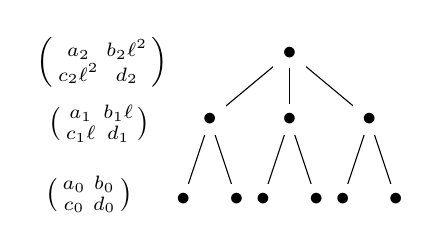
\begin{tikzpicture}[scale=0.225]
\coordinate (A) at (-2,2.5);
\coordinate (B) at (-1,6.5);
\coordinate (C) at (0,10);
\draw (A) node[left]{$\left( \begin{smallmatrix}
a_0 & b_0 \\
c_0 & d_0
\end{smallmatrix} \right) \color{black} $}; %node{$\bullet$};
\draw (B) node[left]{$ \left( \begin{smallmatrix}
a_1 & b_1\ell \\
c_1\ell & d_1
\end{smallmatrix} \right) \color{black} $}; %node{$\bullet$};
\draw (C) node[left]{$ \left( \begin{smallmatrix}
a_2 & b_2\ell^2 \\
c_2\ell^2 & d_2
\end{smallmatrix} \right) \color{black} $}; %node{$\bullet$};
\begin{scope}[yshift=10.5cm,xshift=6.3cm,scale=0.75]
		\coordinate (D) at (0,0);
		\coordinate (E) at (-6,-5);
		\coordinate (F) at (6,-5);
		\coordinate (G) at (-4,-11);
		\coordinate (H) at (-8,-11);
		\coordinate (I) at (4,-11);
		\coordinate (J) at (8,-11);
		\coordinate (K) at (0,-5);
		\coordinate (L) at (-2,-11);
		\coordinate (M) at (2,-11);
		\draw (D) -- (E);
		\draw (D) -- (F);
		\draw (D) -- (K);
		\draw (K) -- (L);
		\draw (K) -- (M);
		\draw (E) -- (H);
		\draw (E) -- (G);
		\draw (F) -- (I);
		\draw (F) -- (J);
		%\coordinate (G) at (E)++(225:3);
		\draw (D) node[fill=white]{$\bullet$};
		\draw (J) node[fill=white]{$\bullet$};
		\draw (E) node[fill=white]{$\bullet$};
		\draw (F) node[fill=white]{$\bullet$};
		\draw (G) node[fill=white]{$\bullet$};
		\draw (H) node[fill=white]{$\bullet$};
		\draw (I) node[fill=white]{$\bullet$};
		\draw (K) node[fill=white]{$\bullet$};
		\draw (L) node[fill=white]{$\bullet$};
		\draw (M) node[fill=white]{$\bullet$};
\end{scope}
\end{tikzpicture}
\end{center}
%\caption{\label{fig:atk:dif:niv:mat} Exemples de matrices du Frobenius obtenues sur les différents niveaux d'un volcan de $\ell$-isogénies}
\end{figure}
%\todo{retravailler cette slide}
%On peut donc comme dans le cas Elkies déterminer le niveau sur lequel se trouve une courbe elliptique dans le volcan d'isogénies dans le cas Atkin. 

\end{frame}

%%%%%%%%%%%%%%%%%%%%%%%%%%%%%%%%%%%%%%%%%%%%%%%%%%%%%%%%%%%%



\begin{frame}
%
%\begin{prop}
%Soient $P,R,R'$ trois points d'une courbe $E$, située au niveau du cratère volcan
%des $\ell$-isogénies, tels que $\langle P,R \rangle = \langle P,R' \rangle= 
%E[\ell^{h+i}]$ avec $i > 0 $ alors $\pi(P,R)=\pi(P,R') $ si et seulement
%si $[\ell^{h}]R=[\ell^{h}]R'$.
%\end{prop}
%\pause 
\begin{figure}
\begin{center}
\begin{tikzpicture}[scale=0.45]
\begin{scope}[yshift=10.5cm,xshift=6.3cm,scale=0.75]
		\coordinate (D) at (0,0);
		\coordinate (E) at (-6,-5);
		\coordinate (F) at (6,-5);
		\coordinate (G) at (-4,-11);
		\coordinate (H) at (-8,-11);
		\coordinate (I) at (4,-11);
		\coordinate (J) at (8,-11);
		\coordinate (K) at (0,-5);
		\coordinate (L) at (-2,-11);
		\coordinate (M) at (2,-11);
		\draw (D) -- (E);
		\draw (D) -- (K);
		\only<2,3>{
		\draw [line width=1.5pt,blue] (D) -- (E);
		\draw [line width=1.5pt,red] (D) -- (K);		
		}
		\draw (D) -- (F);
		\draw (K) -- (L);
		\draw (K) -- (M);
		\draw (E) -- (H);
		\only<3>{
		\draw [line width=1.5pt,red] (K) -- (M);
		\draw [line width=1.5pt,blue] (E) -- (H);
		}
		
		\draw (E) -- (G);
		\draw (F) -- (I);
		\only<4>{
		\draw [line width=1.5pt,red] (D) -- (K);
		\draw [line width=1.5pt,red] (K) -- (M);
		\draw [line width=1.5pt,blue] (D) -- (F);
		\draw [line width=1.5pt,blue] (F) -- (I);
		}
		\draw (F) -- (J);
		\draw (D) node[fill=white]{$E$};
		\draw (K) node[fill=white]{$\bullet$};
		\draw (E) node[fill=white]{$\left( \begin{smallmatrix}7 & 4 
\\4  & 3 \end{smallmatrix} \right)$};
		\only<2>{
		\draw (E) node[fill=white]{$\color{blue}  \left( \begin{smallmatrix}7 & 4 
\\4  & 3 \end{smallmatrix} \right)$};		
		}
		\draw (F) node[fill=white]{$\left( \begin{smallmatrix}3 & 4 
\\4  & 7 \end{smallmatrix} \right) $};
		\draw (G) node[fill=white]{$\left( \begin{smallmatrix}7 & 12 
\\12  & 3 \end{smallmatrix} \right) $};
		\draw (H) node[fill=white]{$\left( \begin{smallmatrix}15 & 12 
\\4  & 11 \end{smallmatrix} \right) $};
		\only<3>{
		\draw (H) node[fill=white]{$\color{blue} \left( \begin{smallmatrix}15 & 12 
\\4  & 11 \end{smallmatrix} \right) $};
		}
		\draw (L) node[fill=white]{$\bullet $};
		\draw (M) node[fill=white]{$\bullet $};
		\draw (I) node[fill=white]{$\left( \begin{smallmatrix}11 & 12 
\\4 & 15 \end{smallmatrix} \right) $};
		\only<4>{
		\draw (I) node[fill=white]{$\color{blue} \left( \begin{smallmatrix}11 & 12 
\\4 & 15 \end{smallmatrix} \right) $};
		}
		\draw (J) node[fill=white]{$\left( \begin{smallmatrix}3 & 4 
\\4  & 7 \end{smallmatrix} \right) $};
		\coordinate (A) at (12,-5);
		\coordinate (B) at (12,-11);
		\draw (A) node[fill=white]{$\bmod \ell^{h+1}$};
		\draw (B) node[fill=white]{$\bmod \ell^{h+2}$};
\end{scope}
\end{tikzpicture}
\end{center}
\caption{\label{fig:atk:dif:niv:iso} Exemples des isogénies correspondant aux différentes matrices du Frobenius, calculées sur la courbe $E$ au sommet du volcan des $\ell$-isogénies. }
\end{figure}
%\pause
\only<4>{On a alors $\ell^{k-h-1}(\ell-1)$ matrices dans la classe de conjugaison d'une matrice définie modulo $\ell^k$ pour une courbe située au niveau du cratère
}
\end{frame}

%%%%%%%%%%%%%%%%%%%%%%%%%%%%%%%%%%%%%%%%%%%%%%%%%%%%%%%%%%%

\begin{frame}
%Faire une slide disant que l'on a pas la correspondance entre les différentes isogénies descendantes et ensuite embrayer sur les isogénies horizontales...
%De plus on est pas capable de distinguer les isogénies descendantes.

%\begin{prop}
%\label{pro:etu:atk:elk}
%
%Soit $\langle P ,R \rangle = E[\ell^{h-e+1}]$ pour $E$ située au niveau $h-e$ 
%du volcan. Alors pour toute $\ell$-isogénie $\psi$ descendante de domaine $E$ 
%il existe $R'$ tel que $\ker(\psi)=\langle [\ell^{h-e}]R' \rangle$, $\langle P,R' 
%\rangle = E[\ell^{h-e+1}]$ et $ \pi(P,R)= \pi(P,R') $
%\end{prop}
%\pause
%Le Frobenius ne permet pas de distinguer les isogénies descendantes.
\frametitle{Comparison with the Elkies case}
\begin{figure}
\begin{center}

\begin{tikzpicture}[scale=0.290]

\begin{scope}[yshift=10cm]
	\begin{scope}[xshift=4.3cm]
		\coordinate (A) at (-3,0);
		\coordinate (B) at (3,0);
		\coordinate (C) at (270:1.2);
		\draw[-] (A.center) to[bend right=25] (C.center);
		\draw[-,dashed] (A.center) to[bend left=40] (B.center);
		%\draw[-] (A.center) to[bend right=40] (B.center);
		\draw[line width=2.25pt,red] (B.center) to[bend left=25] (C.center);
		%\draw[-,dashed] (B.center) to[bend right] (D.center);
		%\draw[line width=2.5pt,red,->] (A.center) to[bend right=20] (C.center);
			\begin{scope}[xshift=-3cm]% sous volcan de gauche
			\coordinate (A) at (0,0);
			\coordinate (C) at (270:4.2);
			\coordinate (CA) at (265:7.5);
			\coordinate (CB) at (275:7.5);
			\draw (C)--(CA);
			\draw (C)--(CB);
			\draw (A)--(C);
			\draw (CA) node[fill=white]{$\bullet$};
			\draw (CB) node[fill=white]{$\bullet$};
			\draw (A) node[fill=white]{$\bullet$};
			\draw (C) node[fill=white]{$\bullet$};
			\end{scope}
			\begin{scope}[xshift=3cm]% sous volcan de droite
			\coordinate (A) at (0,0);
			\coordinate (C) at (270:4.2);
			\coordinate (CA) at (265:7.5);
			\coordinate (CB) at (275:7.5);
			\draw [line width=1.5pt,red] (C)--(A);
			\draw (C)--(CB);
			\draw (C)--(CA);
			\draw (CA) node[fill=white]{$\bullet$};
			\draw (CB) node[fill=white]{$\bullet$};
			\draw (A) node[fill=white]{$\bullet$};
			\draw (C) node[fill=white]{$\bullet$};
			\end{scope}
			\begin{scope}[yshift=-1.2cm] %sous volcan du bas
			\coordinate (A) at (0,0);
			\coordinate (C) at (270:4.2);
			\coordinate (CA) at (265:7.5);
			\coordinate (CB) at (275:7.5);
			\draw (C)--(CA);
			\draw (C)--(CB);
			\draw [line width=1.5pt,blue] (A)--(C);
			%\draw (CA) node[fill=white]{$\bullet$};
			\coordinate (CAB) at (260:8.5);
			\coordinate (CBB) at (280:8.5);
			\draw (CAB) node {$ \left( \begin{smallmatrix}
					7 & 4 \\
					0 & 3
					\end{smallmatrix} \right) $};
			%\draw (CB) node[fill=white]{$\bullet$};
			\draw (CBB) node{$ \left( \begin{smallmatrix}
					7 & 4 \\
					0 & 3
					\end{smallmatrix} \right) $};
			%c est de la triche ce sont les seules matrices possibles...
			%\draw (A) node{$\bullet$};
			\only<1>{
			\draw [line width=1.5pt,blue] (C)--(CA);
			\draw (CAB) node {$ \color{blue} \left( \begin{smallmatrix}
					7 & 4 \\
					0 & 3
					\end{smallmatrix} \right) $};
			}
			\only<2>{
			\draw [line width=1.5pt,blue] (C)--(CB);
			\draw (CBB) node{$ \color{blue} \left( \begin{smallmatrix}
					7 & 4 \\
					0 & 3
					\end{smallmatrix} \right) $};
			}			
			\draw (C) node[fill=white]{$\bullet$};
			\draw (A) node[fill=white]{$E$};
			
			
			%(C) node[left]{$\mathcal{O}$} node{$\bullet$};			
			
			\end{scope}
			\coordinate (F) at (5,0);
			\coordinate (G) at (5,-7);
			\draw[dashed,<-] (F)--(G) node[midway,right]{$h$};
	\end{scope}
\end{scope}

%faire des fleches courbees avec les indices \ell et \ell^2

\end{tikzpicture}
\end{center}

\caption{\label{fig:elk:dif:niv:mat} Matrices du Frobenius possibles pour une base de $E[8]$ avec le premier vecteur de la base ($P$) fixé et le second ($R$) qui engendre la $4$-isogénie descendante}
\end{figure}

\end{frame}

%%%%%%%%%%%%%%%%%%%%%%%%%%%%%%%%%%%%%%%%%%%%%%%%%%%%%%%%%%%%%


\begin{frame}
\frametitle{An $\ell$-adic Couveignes' algorithm in the Atkin case}
%\begin{figure}
\begin{center}
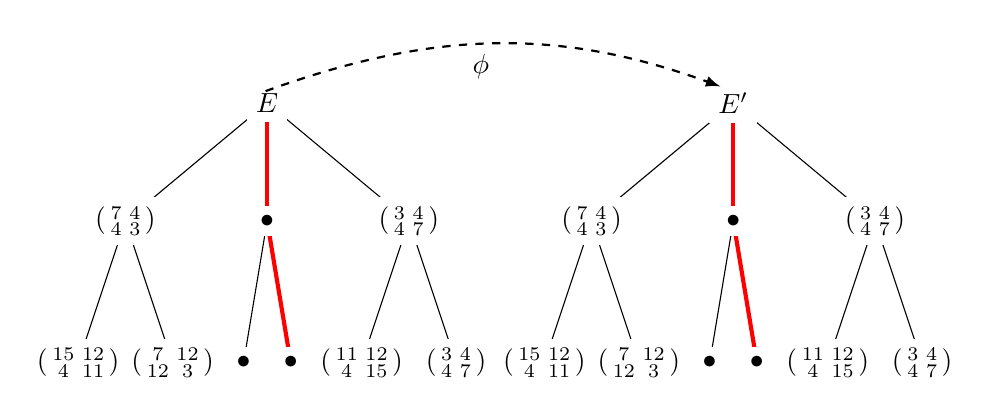
\begin{tikzpicture}[scale=0.40]
\begin{scope}[yshift=10.5cm,xshift=0cm,scale=0.75]
		\coordinate (D) at (0,0);
		\coordinate (E) at (-6,-5);
		\coordinate (F) at (6,-5);
		\coordinate (G) at (-4,-11);
		\coordinate (H) at (-8,-11);
		\coordinate (I) at (4,-11);
		\coordinate (J) at (8,-11);
		\coordinate (K) at (0,-5);
		\coordinate (L) at (-1,-11);
		\coordinate (M) at (1,-11);
		\draw (D) -- (E);
		\draw (D) -- (F);
		\draw [line width=1.5pt,red] (D) -- (K);
		\draw (K) -- (L);
		\draw [line width=1.5pt,red] (K) -- (M);
		\draw (E) -- (H);
		\draw (E) -- (G);
		\draw (F) -- (I);
		\draw (F) -- (J);
		\draw (D) node[fill=white]{$E$};
		\draw (K) node[fill=white]{$\bullet$};
		\draw (E) node[fill=white]{$\left( \begin{smallmatrix}7 & 4 
\\4  & 3 \end{smallmatrix} \right)$};
		\draw (F) node[fill=white]{$\left( \begin{smallmatrix}3 & 4 
\\4  & 7 \end{smallmatrix} \right) $};
		\draw (G) node[fill=white]{$\left( \begin{smallmatrix}7 & 12 
\\12  & 3 \end{smallmatrix} \right) $};
		\draw (H) node[fill=white]{$\left( \begin{smallmatrix}15 & 12 
\\4  & 11 \end{smallmatrix} \right) $};
		\draw (L) node[fill=white]{$\bullet $};
		\draw (M) node[fill=white]{$\bullet $};
		\draw (I) node[fill=white]{$\left( \begin{smallmatrix}11 & 12 
\\4 & 15 \end{smallmatrix} \right) $};
		\draw (J) node[fill=white]{$\left( \begin{smallmatrix}3 & 4 
\\4  & 7 \end{smallmatrix} \right) $};
		%\coordinate (A) at (12,-5);
		%\coordinate (B) at (12,-11);
		%\draw (A) node[fill=white]{$\bmod \ell^{h+1}$};
		%\draw (B) node[fill=white]{$\bmod \ell^{h+2}$};
\end{scope}
\begin{scope}[yshift=10.5cm,xshift=14.8cm,scale=0.75]
		\coordinate (D) at (0,0);
		\coordinate (E) at (-6,-5);
		\coordinate (F) at (6,-5);
		\coordinate (G) at (-4,-11);
		\coordinate (H) at (-8,-11);
		\coordinate (I) at (4,-11);
		\coordinate (J) at (8,-11);
		\coordinate (K) at (0,-5);
		\coordinate (L) at (-1,-11);
		\coordinate (M) at (1,-11);
		\draw (D) -- (E);
		\draw (D) -- (F);
		\draw [line width=1.5pt,red] (D) -- (K);
		\draw (K) -- (L);
		\draw [line width=1.5pt,red] (K) -- (M);
		\draw (E) -- (H);
		\draw (E) -- (G);
		\draw (F) -- (I);
		\draw (F) -- (J);
		\draw (D) node[fill=white]{$E'$};
		\draw (K) node[fill=white]{$\bullet$};
		\draw (E) node[fill=white]{$\left( \begin{smallmatrix}7 & 4 
\\4  & 3 \end{smallmatrix} \right)$};
		\draw (F) node[fill=white]{$\left( \begin{smallmatrix}3 & 4 
\\4  & 7 \end{smallmatrix} \right) $};
		\draw (G) node[fill=white]{$\left( \begin{smallmatrix}7 & 12 
\\12  & 3 \end{smallmatrix} \right) $};
		\draw (H) node[fill=white]{$\left( \begin{smallmatrix}15 & 12 
\\4  & 11 \end{smallmatrix} \right) $};
		\draw (L) node[fill=white]{$\bullet $};
		\draw (M) node[fill=white]{$\bullet $};
		\draw (I) node[fill=white]{$\left( \begin{smallmatrix}11 & 12 
\\4 & 15 \end{smallmatrix} \right) $};
		\draw (J) node[fill=white]{$\left( \begin{smallmatrix}3 & 4 
\\4  & 7 \end{smallmatrix} \right) $};
		%\coordinate (A) at (12,-5);
		%\coordinate (B) at (12,-11);
		%\draw (A) node[fill=white]{$\bmod \ell^{h+1}$};
		%\draw (B) node[fill=white]{$\bmod \ell^{h+2}$};
		\coordinate (A) at (-19.8,0.5);
		\coordinate (B) at (0,0.5);
		%\draw [->] (A) --(B);
		%\draw[bend right =20] (A)--(B);
		\draw[dashed,thick,-latex,shorten >=5pt] (A) to[bend left=20] node[below left] {$\phi$} (B);
\end{scope}
\end{tikzpicture}
\end{center}
%\end{figure}
Once the image by $\phi$ of one of the two bases point of $E[\ell^k]$ is 
determined, then the matrix that represents the Frobenius determines the 
descending isogenies generated by the second basis point. 
%Une fois que l'image par $\phi$ d'un des deux points de la base de la $\ell^k$-torsion a été déterminé alors la forme de la matrice du Frobenius détermine les $\ell$-isogénies descendantes engendrées par le second point de la base.
\end{frame}

%%%%%%%%%%%%%%%%%%%%%%%%%%%%%%%%%%%%%%%%%%%%%%%%%%%%%%%

\begin{frame}

\bluebox{Towards an $\ell$-adic Couveignes' algorithm (Atkin case)}{
\begin{algorithmic}[1]
\REQUIRE $E, E'$ two $r$-isogenous curves on $\mathbb{F}_{q}$ 
\ENSURE $\phi: E \rightarrow E'$ of degree $r$
\end{algorithmic}}

\bluebox{}{\textbf{Fact:}$\pi(P,R)=\pi(\phi(P),\phi(R))$ and $\pi(P,R)=\pi(P,R')$ iff $[\ell^h]R=[\ell^h]R'$.}

\begin{enumerate}
\item Select the least $k$ such that $\ell^{2k}>4r$.
\medskip
\item Compute $\langle P , Q \rangle = E[\ell^k]$ and $\langle P' , Q' \rangle = E'[\ell^k]$
%\item Deduce $\to$ $\langle{\color{red}P},{\color{blue}Q}\rangle=E[\ell^k]$ and $\langle{\color{red}P'},{\color{blue}Q'}\rangle=E'[\ell^k]$;
\medskip
\item Compute the matrix $\pi(P,Q)$;
\medskip
\item For each point $S'$ of order $\ell^k$ in $E'$: \hfill\only<2>{$O(r)$}
\begin{enumerate}
\medskip
  \item Computation of $R'$ such that $\pi(S',R')=\pi(P,Q)$ \hfill\only<2>{$O(\ell^4 r)$}
  \medskip
  \item For each point $U' \in E'$ such that $[\ell^h]R'=[\ell^h]U'$ \hfill\only<2>{$O(\sqrt{r})$}
  \begin{enumerate}

  \item Compute the interpolation polynomial
    $L$ sending\\
    $P\mapsto S'$ and $Q\mapsto U'$;
\hfill\only<2>{$\tilde{O}(r \ell^{O(1)})$}
	\item Use a  rational reconstruction  algorithm 
    to compute a rational
    fraction $F$ of degrees~$(r, r-1)$;
\hfill\only<2>{$\tilde{O}(r)$}
  \item If $F$ defines an isogeny of degree $r$, return it and
    stop.
  \end{enumerate}

\end{enumerate}
\end{enumerate}

\end{frame}

%%%%%%%%%%%%%%%%%%%%%%%%%%%%%%%%%%%%%%%%%%%%%%%%%%%%%%%%%%%%%

%%%%%%%%%%%%%%%%%%%%%%%%%%%%%%%%%%%%%%%%%%%%%%%%%%%%%%%%%%%%


\begin{frame}
  \frametitle{Towers of field extensions}

  \bluebox{Computing in towers of field extensions}{
  \begin{itemize}
%   \item We work on $\mathbb{F}_q$ such that $E[\ell] \subset E(\mathbb{F}_q)$,
	\item Torsion points are not defined in $\mathbb{F}_q$, in general.	
	\item We work in $\ell$-adic extensions of $\mathbb F_q$
        using constructions from [De~Feo,~Doliskani, Schost '13], [Doliskani,~Schost '15] where in particular we have a fast computation of the Frobenius.
	
  \end{itemize}
 	
  }

\end{frame}

%%%%%%%%%%%%%%%%%%%%%%%%%%%%%%%%%%%%%%%%%%%%%%%%%%%%%%%%%%%%

\begin{frame}
\frametitle{Experiments}
The algorithm has been implemented on SageMath v7.1 for the case of $\ell=2$, the code is available on GitHub: \url{https://github.com/Hugounenq-Cyril/Two_curves_on_a_volcano}
\begin{figure}[hbtp]
\centering
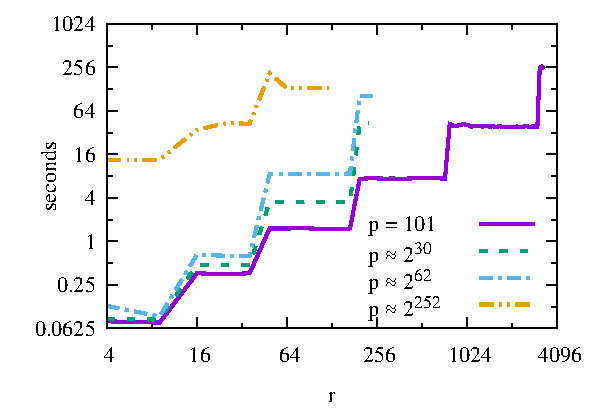
\includegraphics[scale=0.8]{Images/graphe-101-149-269.pdf}
\end{figure}
\end{frame}


%%%%%%%%%%%%%%%%%%%%%%%%%%%%%%%%%%%%%%%%%%%%%%%%%%%%%%%%%%%% 

\begin{frame}
\frametitle{Conclusion}
\bluebox{Contribution}{
\begin{itemize}
\item New tools for navigating isogeny volcanoes. 

\item A faster variant of Couveignes' algorithm only with Elkies primes.

\end{itemize}
}
\bluebox{Future work}{
\begin{itemize}
\item Compare implementation to other algorithms (esp. Lercier-Sirvent).
% \item Directly generalize to curves not on the crater.
\item Give an analogous algorithm for Atkin primes with a quadratic complexity 
(only subcubic has been done).
\item Estimate the cost of the computation of endomorphism rings with the study of the action of the Frobenius and implement it.
\item Analyze our techniques to navigate the volcano in other
  settings: point counting, , Hilbert
  class polynomials, modular polynomials.
\end{itemize}}

%Code available on GitHub: \url{https://github.com/Hugounenq-Cyril/Two_curves_on_a_volcano}
\end{frame}

% \begin{frame} 

% \bibliography{Biblio}
% \end{frame}

\setbeamertemplate{headline}{\relax}
\setbeamertemplate{footline}{\relax}
\begin{frame}
\begin{center}
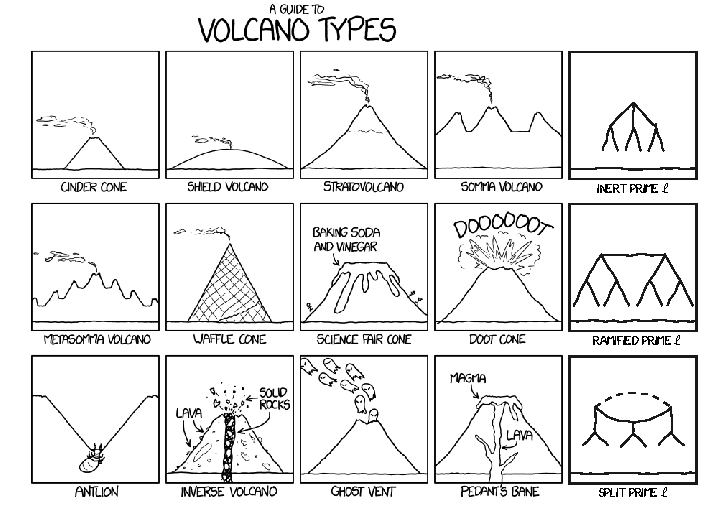
\includegraphics[width=.9\hsize]{Images/volcan}
\end{center}
\tiny Modified from  \href{http://xkcd.com/1714/}{xkcd.com/1714}
\end{frame}

%%%%%%%%%%%%%%%%%%%%%%%%%%%%%%%%%%%%%%%%%%%%%%%%%%%%%%%%%%%%

\begin{frame}
\frametitle{Technical details: Improving interpolation with Frobenius}
%$A$ the polynomial that interpolates the isogeny according to the mappings $\red P \rightarrow \color{red} u P' $, $\blu Q \rightarrow \color{blue}v Q'$  and $\color{red} P' \in  E'[\ell^k]_{\lambda}$, $\color{blue} Q' \in  E'[\ell^k]_{\mu} \color{black}$.

%$T$ the polynomial that interpolates the isogeny according to the mapping \[P \mapsto a P \quad Q \mapsto bQ \quad \textit{with } a,b \wedge \ell = 1.\]
We want to compute an $\mathbb{F}_q$ \textbf{rational} isogeny, then for each interpolation polynomial candidate $L$ we have for $R \in E[\ell^k]$: 
\[\pi(L(x(R)))=L(x(\pi(R))),\]
and in particular with $\color{red} P \in  E[\ell^k]_{\lambda}$, $\color{blue} Q \in  E[\ell^k]_{\mu} \color{black}$:
\[\pi(L(x(\red P)))=L(x(\color{red} \lambda P \color{black}))) \quad \pi(L(x(\blu Q)))=L(x(\color{blue} \mu Q \color{black}))).\]
\pause
As suggested by [Couveignes,96] we construct $L$ separately from the representatives points of an orbit under the action of the Frobenius: 
\[
\{ {\boldmath \color{red} \textbf{P}} \unboldmath , \pi(\red P), \pi^2(\red P), \cdots \color{black} \}  
\]
\[
\{ {\boldmath \color{blue} \textbf{Q}} \unboldmath , \pi(\blu Q), \pi^2(\blu Q), \cdots \color{black} \}  
\]
\[
\cdots
\]
and then we use the Chinese  Remainder Theorem to get $L$.

\end{frame}

%%%%%%%%%%%%%%%%%%%%%%%%%%%%%%%%%%%%%%%%%%%%%%%%%%%%%%%%%%%% 
%%%%%%%%%%%%%%%%%%%%%%%%%%%%%%%%%%%%%%%%%%%%%%%%%%%%%%%%%%%% 


\begin{frame}
\frametitle{Technical details: Improving interpolation with Frobenius}
\begin{figure}[h]
\begin{center}

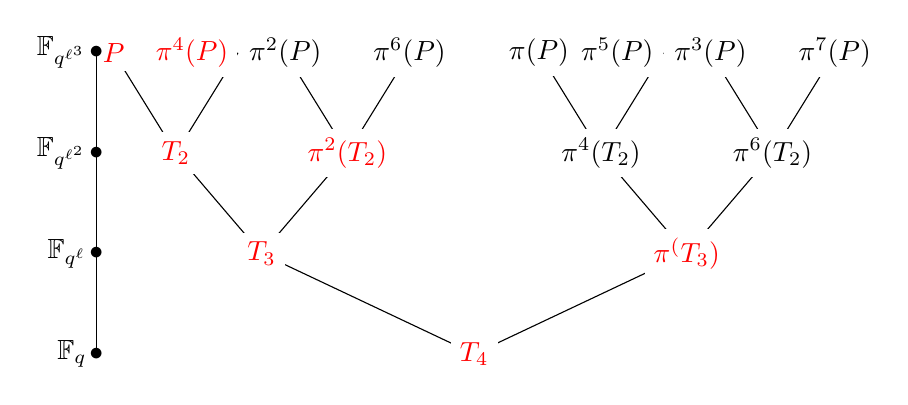
\begin{tikzpicture}[scale=0.3]
        \coordinate (A) at (0,0);
        \coordinate (AB) at (-9,4.25);
		\coordinate (AC) at (9,4.25);
		\draw (A)--(AB);
		\draw (A)--(AC);
		\draw (A) node[fill=white]{$\color{red}{T_4}$};
		

		\coordinate (ABA) at (-12.63,8.5);
		%\coordinate (ABA) at (-11.63,8.5);
		
		\draw (ABA)--(AB);
		
		\coordinate (ABAb) at (-15.26,12.75);
		%\coordinate (ABAb) at (-14.26,12.75);
		
		\draw (ABA)--(ABAb);
		\draw (ABAb) node[fill=white]{$\color{red}{P}$};
		
		\coordinate (ABAa) at (-10,12.75);
		%\coordinate (ABAa) at (-9,12.75);
		
		
		\draw (ABA)--(ABAa);
		\draw (ABA) node[fill=white]{$\color{red}{T_2}$};
		\draw (ABAa) node[fill=white][left]{$\color{red}{\pi^4(P)}$};%ancien \pi(T)
		
		\coordinate (ACA) at (-5.37,8.5);
		%\coordinate (ACA) at (-6.37,8.5);
		
		
		\draw (AB)--(ACA);
		\draw (AB) node[fill=white]{$\color{red}{T_3}$};
		\coordinate (ACAa) at (-8,12.75);
		%\coordinate (ACAa) at (-9,12.75);
		
		
		\draw (ACA)--(ACAa);
		\draw (ACAa) node[fill=white]{$\pi^2(P)$};%ancien \pi^2(T)
		
		\coordinate (ACAb) at (-2.74,12.75);
		%\coordinate (ACAb) at (-3.74,12.75);
		
		
		\draw (ACA)--(ACAb);
		\draw (ACAb) node[fill=white]{$\pi^6(P)$};%ancien \pi^3(T)
		\draw (ACA) node[fill=white]{$\color{red}{\pi^2(T_2)}$};% ancien \pi^2(T_2)
		
		\begin{scope}[xshift=18cm]
		\coordinate (ABA) at (-12.63,8.5);
		%\coordinate (ABA) at (-11.63,8.5);

		\draw (ABA)--(AC);
		
		\coordinate (ABAb) at (-15.26,12.75);
		%\coordinate (ABAb) at (-14.26,12.75);
		
		\draw (ABA)--(ABAb);
		\draw (ABAb) node[fill=white]{$\pi(P)$};%ancien \pi^4(T)
		
		\coordinate (ABAa) at (-10,12.75);
		%\coordinate (ABAa) at (-9,12.75);
		
		
		\draw (ABA)--(ABAa);
		\draw (ABAa) node[fill=white,left]{$\pi^5(P)$};%ancien \pi^5(T)
		\draw (ABA) node[fill=white]{$\pi^4(T_2)$};%ancien \pi^4(T_2)
		
		\coordinate (ACA) at (-5.37,8.5);
		%\coordinate (ACA) at (-6.37,8.5);
		
		
		\draw (AC)--(ACA);
		\draw (AC) node[fill=white]{$\color{red}{\pi^(T_3)}$};%ancien \pi^4(T_3)
		
		\coordinate (ACAa) at (-8,12.75);
		%\coordinate (ACAa) at (-9,12.75);
		
		
		\draw (ACA)--(ACAa);
		\draw (ACAa) node[fill=white]{$\pi^3(P)$};%ancien \pi^6(T)
		
		\coordinate (ACAb) at (-2.74,12.75);
		%\coordinate (ACAb) at (-3.74,12.75);
		
		
		\draw (ACA)--(ACAb);
		\draw (ACAb) node[fill=white]{$\pi^7(P)$};%ancien \pi^7(T)	
		\draw (ACA) node[fill=white]{$\pi^6(T_2)$};%ancien \pi^6(T_2)	
		\end{scope}
		
		\coordinate (A1) at (-16,0);
		\coordinate (A2) at (-16,4.25);
		\coordinate (A3) at (-16,8.5);
		\coordinate (A4) at (-16,12.75);
		\draw (A1)--(A2)--(A3)--(A4);
		\draw (A1) node{$\bullet$};
		\draw (A2) node{$\bullet$};
		\draw (A3) node{$\bullet$};
		\draw (A4) node{$\bullet$};
		\draw (A1) node[left]{$\mathbb{F}_q$};
		\draw (A2) node[left]{$\mathbb{F}_{q^\ell}$};
		\draw (A3) node[left]{$\mathbb{F}_{q^{\ell^2}}$};
		\draw (A4) node[left]{$\mathbb{F}_{q^{\ell^3}}$};
\end{tikzpicture}

\end{center}
\end{figure}
Elements of the binary tree we need for the computation of the interpolation polynomial.
\end{frame}


%%%%%%%%%%%%%%%%%%%%%%%%%%%%%%%%%%%%%%%%%%%%%%%%%%%%%%%%%%%%%%%%%%%%%%

\begin{frame}
\frametitle{Bonus: ascending horizontal points}
\begin{figure}
\begin{center}
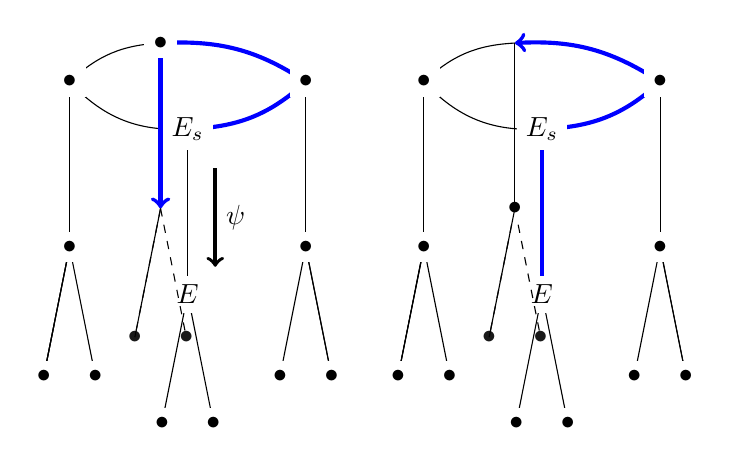
\begin{tikzpicture}[scale=0.50]
\begin{scope}%[yshift=10cm]
	\begin{scope}[xshift=4.3cm]
		%Cratere
		\node (A) at (-3,0) {$\bullet$};
		\node (B) at (3,0) {$\bullet$};
		\node (C) at (270:1.2) {$\bullet$};
		\node (D) at (125:1.2) {$\bullet$};
		\draw[-] (A.center) to[bend right=25] (C.center);
		\draw[-] (D.center) to[bend right=20] (A.center);	
		\draw[line width=1.5pt,blue,->] (D.center) to[bend left=18] (B.center);
		
		\draw[line width=1.5pt,blue,->] (C.center) to[bend right=20] (B.center); 
		%\node (F) at (1.5,-0.5) {$\color{blue} \mu$};	

		
			\begin{scope}[xshift=-3cm] %sous-volcan de gauche
			\coordinate (A) at (0,0);
			\coordinate (C) at (270:4.2);
			\coordinate (CA) at (265:7.5);
			\coordinate (CB) at (275:7.5);
			\draw (C)--(CA);
			
			\draw (C)--(CB);
			\draw (A)--(C);
			\draw  (C)--(A);
			\draw  (C)--(CA);
			%just to have a 6th slide
			
			\draw (C)--(A);
			\draw (C)--(CA);
			\draw (A) node[fill=white]{$\bullet$};
			\draw (C) node[fill=white]{$\bullet$};
			\draw (CA) node[fill=white]{$\bullet$};
			\draw (CB) node[fill=white]{$\bullet$};
			\end{scope}
			\begin{scope}[xshift=3cm] %sous-volcan de droite
			\coordinate (A) at (0,0);
			\coordinate (C) at (270:4.2);
			\coordinate (CA) at (265:7.5);
			\coordinate (CB) at (275:7.5);
			\draw (C)--(CA);
			\draw (C)--(CB);
			\draw (A)--(C);
			\draw (C)--(CB);
			\draw (A)--(C);
			\draw (A) node[fill=white]{$\bullet$};
			%\only<2-3>{\draw (A) node[fill=yellow!50!white,shape=circle]{$E_1$};}
			\draw (C) node[fill=white]{$\bullet$};
			\draw (CA) node[fill=white]{$\bullet$};
			\draw (CB) node[fill=white]{$\bullet$};
			\end{scope}
			\begin{scope}[yshift=-1.2cm] %sous volcan du bas
			\coordinate (A) at (0,0);
			\coordinate (C) at (270:4.2);
			\coordinate (CA) at (265:7.5);
			\coordinate (CB) at (275:7.5);
			\draw (C)--(CA);
			\draw (C)--(CB);
			\draw (A)--(C);
			\draw (A) node[fill=white]{$E_s$};
			%\only<1>{\draw (A) node[fill=yellow!50!white,shape=circle]{$E$};}
			\draw (C) node[fill=white]{$E$};
			\draw (CA) node[fill=white]{$\bullet$};
			\draw (CB) node[fill=white]{$\bullet$};
			\coordinate (G) at (0.7,-1);
			\coordinate (H) at (0.7,-3.5);
			\draw [line width=1.3pt,black,->] (G)--(H) node[midway,right] {$\psi$};
			\end{scope}
			\begin{scope}[shift={(D)}] %sous volcan du haut
			\coordinate (A) at (0,0);
			\coordinate (C) at (270:4.2);
			\coordinate (CA) at (265:7.5);
			\coordinate (CB) at (275:7.5);
			\draw [dashed] (C)--(CA);
			\draw [dashed] (C)--(CB);
			\draw [dashed] (A)--(C);
			%\draw (C) node[color=black!90]{$\bullet$};
			\draw (CA) node[color=black!90]{$\bullet$};
			\draw (CB) node[color=black!90]{$\bullet$};
			%\only<3>{
			\draw [line width=1.5pt,blue,<-] (C)--(A);
			\draw (C)--(CA);
			\draw (A) node[fill=white]{$\bullet$};
			\end{scope}
	\end{scope}
\end{scope}
\begin{scope}[xshift=9cm] %volcan de droite
	\begin{scope}[xshift=4.3cm]
		%Cratere
		\node (A) at (-3,0) {$\bullet$};
		\node (B) at (3,0) {$\bullet$};
		\node (C) at (270:1.2) {$\bullet$};
		\node (D) at (125:1.2) {};
		\draw[-] (A.center) to[bend right=25] (C.center);
		\draw[-] (D.center) to[bend right=20] (A.center);	
		\draw[line width=1.5pt,blue,<-] (D.center) to[bend left=18] (B.center);
		
		\draw[line width=1.5pt,blue,->] (C.center) to[bend right=20] (B.center); 
		%\node (F) at (1.5,-0.5) {$\color{blue} \mu$};	

		
			\begin{scope}[xshift=-3cm] %sous-volcan de gauche
			\coordinate (A) at (0,0);
			\coordinate (C) at (270:4.2);
			\coordinate (CA) at (265:7.5);
			\coordinate (CB) at (275:7.5);
			\draw (C)--(CA);
			
			\draw (C)--(CB);
			\draw (A)--(C);
			\draw  (C)--(A);
			\draw  (C)--(CA);
			%just to have a 6th slide
			
			\draw (C)--(A);
			\draw (C)--(CA);
			\draw (A) node[fill=white]{$\bullet$};
			\draw (C) node[fill=white]{$\bullet$};
			\draw (CA) node[fill=white]{$\bullet$};
			\draw (CB) node[fill=white]{$\bullet$};
			\end{scope}
			\begin{scope}[xshift=3cm] %sous-volcan de droite
			\coordinate (A) at (0,0);
			\coordinate (C) at (270:4.2);
			\coordinate (CA) at (265:7.5);
			\coordinate (CB) at (275:7.5);
			\draw (C)--(CA);
			\draw (C)--(CB);
			\draw (A)--(C);
			\draw (C)--(CB);
			\draw (A)--(C);
			\draw (A) node[fill=white]{$\bullet$};
			%\only<2-3>{\draw (A) node[fill=yellow!50!white,shape=circle]{$E_1$};}
			\draw (C) node[fill=white]{$\bullet$};
			\draw (CA) node[fill=white]{$\bullet$};
			\draw (CB) node[fill=white]{$\bullet$};
			\end{scope}
			\begin{scope}[yshift=-1.2cm] %sous volcan du bas
			\coordinate (A) at (0,0);
			\coordinate (C) at (270:4.2);
			\coordinate (CA) at (265:7.5);
			\coordinate (CB) at (275:7.5);
			\draw (C)--(CA);
			\draw (C)--(CB);
			\draw [line width=1.5pt,blue](A)--(C);
			\draw (A) node[fill=white]{$E_s$};
			%\only<1>{\draw (A) node[fill=yellow!50!white,shape=circle]{$E$};}
			\draw (C) node[fill=white]{$E$};
			\draw (CA) node[fill=white]{$\bullet$};
			\draw (CB) node[fill=white]{$\bullet$};
			\end{scope}
			\begin{scope}[shift={(D)}] %sous volcan du haut
			\coordinate (A) at (0,0);
			\coordinate (C) at (270:4.2);
			\coordinate (CA) at (265:7.5);
			\coordinate (CB) at (275:7.5);
			\draw [dashed] (C)--(CA);
			\draw [dashed] (C)--(CB);
			\draw [dashed] (A)--(C);
			\draw (C) node[fill=white]{$\bullet$};
			\draw (CA) node[color=black!90]{$\bullet$};
			\draw (CB) node[color=black!90]{$\bullet$};
			%\only<3>{
			\draw (C)--(A);
			\draw (C)--(CA);
			\end{scope}
	\end{scope}
\end{scope}

\end{tikzpicture}
\end{center}
\caption{ Construction of an ascending horizontal point from a point $P \in 
E_s$ of order $2^3$ such that $[2]P$ is an horizontal point and $\psi: E_s 
\rightarrow E$ is a descending $2$-isogeny.} 
%à partir d'un point $P \in E_s$ d'ordre $2^3$ tel que $[2]P$ soit 
%horizontal de direction $\color{blue}{\mu}$ et $\psi:E_s \rightarrow E$ une 
%$2$-isogénie descendante.}
\end{figure}
\end{frame}

%%%%%%%%%%%%%%%%%%%%%%%%%%%%%%%%%%%%%%%%%%%%%%%%%%%%%%%%%%%%%
\begin{frame}
%\section{Computation of endomorphism rings}
\frametitle{Computation of endomorphism rings}
\begin{prop} [Silverman, '86]
Soit $E$ une courbe elliptique alors son anneau d'endomorphismes $\mathrm{End}(E)$ est isomorphe à un ordre $\mathcal{O}$ défini dans un corps de nombre quadratique imaginaire noté ici $K$. 
\end{prop}

\begin{prop}
Soit $E$ une courbe elliptique ordinaire, alors 
\[
\mathbb{Z} \left[ \pi \right] \subset \mathcal{O} \subset \mathcal{O}_K
\] 
avec $\mathcal{O}_K$ l'anneau des entiers de $K$. %le corps de nombre quadratique imaginaire tel que $\mathcal{O} \subset K$
\end{prop}

\begin{defi}[Conducteur]
On note $g=[\mathcal{O}_K:\mathbb{Z}[\pi]]$ le conducteur de $\mathbb{Z}[\pi]$. %et $f$ le conducteur de $[\mathcal{O}_K:\mathcal{O}]$.
\end{defi}
\end{frame}

\begin{frame}
\begin{defi}[Discriminant]
On note $d_{\pi}$ (resp. $d_K$) le discriminant de l'ordre $\mathbb{Z}\left[ \pi \right]$ (resp. $\mathcal{O}_K$).
\end{defi}
En particulier: $d_{\pi}=g^2d_K$

\begin{prop}[Preciser source vu dans Fouquet '01]
Il existe un entier $a$ tel que \[\mathcal{O}_K=\mathbb{Z} \left[ \frac{\pi-a}{g} \right] \quad \text{et} \quad (X-a)^2=X^2-t_{\pi}X+q \bmod g \]
\end{prop}

\end{frame}

\begin{frame}


\bluebox{Algorithm to compute the endomorphism ring of $E$ [Kohel '96]}{
\begin{algorithmic}[1]
\REQUIRE $d_{\pi}$ the discriminant of the Elliptic curve $E$; 
\ENSURE $\mathcal{O}$ the endomorphism ring of $E$
\end{algorithmic}}

\begin{enumerate}
\item Compute the prime factorization of $d_{\pi}$ and deduce from it the conductor  $g=\prod_{i=1}^j\ell_i^{t_i}$ such that $d_{\pi}=g^2d_K$ and $a$ such that $\mathcal{O}_K=\mathbb{Z} \left[ \frac{\pi-a}{g} \right] $ 
\item For each $\ell_i$:
\begin{enumerate}
\item Compute $s_i= v_{\ell_i}([\mathcal{O}:\mathbb{Z}[\pi]]) $
\end{enumerate}
\item Return $\mathcal{O}=\mathbb{Z}+\left( (\pi-a)/\prod_{i=1}^j\ell_i^{s_i} \right) \mathbb{Z}$
\end{enumerate}

\bluebox{Previous work on the computation of $v_{\ell_i}([\mathcal{O}:\mathbb{Z}[\pi]]) $}{
\begin{itemize}
\item Kohel (1996) work with modular polynomials (variants with division polynomials, and ideal class group)
\item Bisson-Sutherland (2009) enumerations of relations built from isogeny cycles
\end{itemize}
}
%Parler de Kohel (Vu dans la thèse de Mireille 1) Methode par les polynomes de division, 2) polynomes modulaires 3) Methode par les ideaux 3.a) enumeration 3.b) groupe de classe d ideaux )

%Parler de Bisson Sutherland (Utilise les cycles d'isogénies et les relations qui donnent un endomorphisme)}
\end{frame}

%%%%%%%%%%%%%%%%%%%%%%%%%%%%%%%%%%%%%%%%%%%%%%%%%%%%%%%%%%%%%
\begin{frame}
%A l'aide des propositions sur les formes de la matrice dans le cas Atkin et 
%Elkies on peut savoir à quel niveau du volcan se trouve une courbe elliptique.
%
% 
%Faire une slide qui parle de ça 
%Il faut juste dire comment l'on distingue un cas Atkin d'un cas Elkies...
%Faire une estimation à la louche

\bluebox{Algorithm to compute the endomorphism ring of $E$}{
\begin{algorithmic}[1]
\REQUIRE $d_{\pi}$ the discriminant of the Elliptic curve $E$; 
\ENSURE $\mathcal{O}$ the endomorphism ring of $E$
\end{algorithmic}}

\bluebox{}{\textbf{Fact:} For $\langle P, R \rangle = E[\ell_i^{r_i+1}]$ with $r_i=\lfloor v_{\ell_i}(d_{\pi})/2 \rfloor $ from  $\pi(P,R)$ we deduce $v_{\ell_i}([\mathcal{O}:\mathbb{Z}[\pi]])$.}

\begin{enumerate}
\item Compute from $d_{\pi}$ the prime factorization of the conductor $g=\prod_{i=1}^j\ell_i^{t_i}$ of $\mathbb{Z}[\pi]$ and $a$ such that $\mathcal{O}_K=\mathbb{Z} \left[ \frac{\pi-a}{g} \right] $ 
\item For each $\ell_i$:
\begin{enumerate}
\item Compute $\langle P , Q \rangle = E[\ell_i^{r_i+1}]$
\medskip
\item Determine from $d_{\pi}$ if $\ell_i$ is an Atkin or an Elkies prime 
\medskip 
\item Compute $\pi(P,Q)$ and deduce from it $s_i=v_{\ell_i}([\mathcal{O}:\mathbb{Z}[\pi]])$ 
\end{enumerate}
\item Return $\mathcal{O}=\mathbb{Z} + \left( (\pi-a)/ \prod_{i=1}^j\ell_i^{s_i} \right) \mathbb{Z}$
\end{enumerate}
\end{frame}

\begin{frame}
Parler de la représentation univariée et bivariée, dire que les calculs sont toujours plus rapide en univariée, montrer le passage d'une représentation bivariée à univariée. Dire que l'on peut ajouter des étages à la volée. Mentionner que l'on a des bonnes complexités pour le Frobenius en particulier.

\begin{equation*}
\begin{alignedat}{1}
 G(x_k) &= G_0(x_k)+ G_1(x_k^\ell)+x_kG_2(x_k^\ell)+ \cdots + x_k^{\ell-1} G_{\ell}(x_k^{\ell})\\
&= G_0(x_k)+G_1(x_{k-1})+x_kG_2(x_{k-1})+ \cdots x_k^{\ell-1}G_{\ell}(x_{k-1})
\end{alignedat}
\end{equation*}
\end{frame}

\begin{frame}
\begin{exe}
Soit $\mathbb{F}_q, \mathsf{F}_1, \mathsf{F}_2, \cdots, \mathsf{F}_k$ une tour d'extensions $5$-adiques telle que $\mathbb{F}_q \cong \mathsf{F}_1$, soit $\alpha \in \mathsf{F}_4$ qui s'écrit dans la $\mathbb{F}_q$ base monomiale de $\mathsf{F}_4$:
\begin{equation}
\label{eq:exe:mon}
\alpha_0 + \alpha_5x_4^5+ \alpha_{10}x_4^{10} + \alpha_{15}x_4^{15} + \cdots + \alpha_{5k}x_4^{5k} + \cdots + \alpha_{120}x_4^{120} 
\end{equation} 
alors $\alpha$ s'écrit de la façon suivante dans la base bivariée de $\mathsf{F}_4$:
\begin{equation}
\label{eq:exe:biv}
\alpha_0 + \alpha_5x_3^1+ \alpha_{10}x_3^{2} + \alpha_{15}x_3^{3} + \cdots + \alpha_{5k}x_3^{k} + \cdots + \alpha_{120}x_3^{24}. 
\end{equation} 
 Ainsi on voit que $\alpha$ est aussi un élément de $\mathsf{F}_3$. Le passage de la représentation de $\alpha$ de \eqref{eq:exe:mon} à \eqref{eq:exe:biv} correspond à une \emph{descente}, l'opération inverse est elle un \emph{relèvement}.
 
 Par contre pour $\beta$ un élément de $\mathsf{F}_4$ écrit de la façon suivante dans la base monovariée:
 \begin{equation*}
 \beta_0 + \beta_1 x_4+ \cdots +\beta_{5k}x_4^{5k} + \beta_{5k+1}x_4^{5k+1}+\beta_{5k+2}x_4^{5k+2}+ \beta_{5k+3}x_4^{5k+3}+ \beta_{5k+4}x_4^{5k+4}+ \cdots + \beta_{124}x_4^{124}
 \end{equation*}
l'écriture de $\beta$ dans la base bivariée est: 
 \begin{equation*}
  \beta_0 + \beta_1 x_4+ \cdots + x_3^{k}(\beta_{5k}+\beta_{5k+1} x_4 + \beta_{5k+2} x_4^2 + \beta_{5k+3} x_4^3 + \beta_{5k+4}x_3^4)+ \cdots + \beta_{124}x_3^{24}x_4^{4}.
 \end{equation*}
 On voit ici que $\beta \notin \mathsf{F}_3$ et donc on ne peut le faire descendre dans la tour d'extension mais seulement s'arrêter à cette écriture dans la base bivariée.
\end{exe}

\end{frame}


\end{document}

%%%%%%%%%%%%%%%%%%%%%%%%%%%%%%%%%%%%%%%%%%%%%%%%%%%%%%%%%%%%

\begin{frame}
\frametitle{Motivation}
How to communicate securely on a channel that is not ?
%mettre une image de communication entre deux personnes
\only<1-1>{
\begin{center}
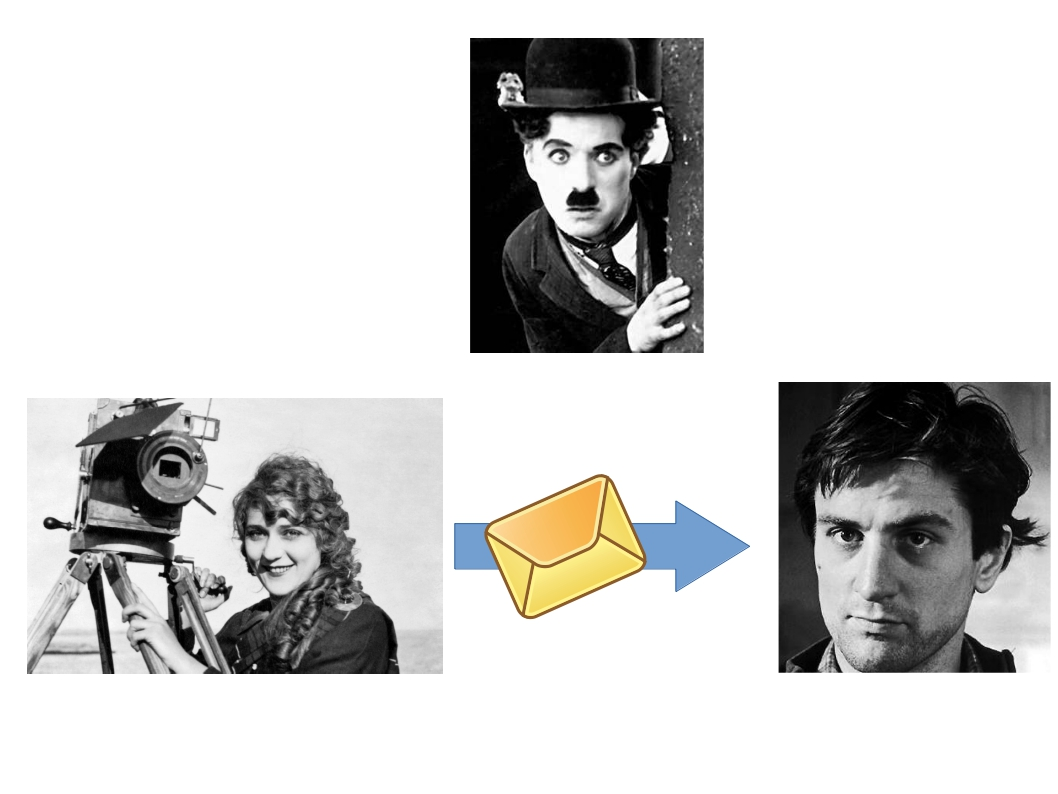
\includegraphics[scale=0.30]{Images/communication_Alice_Bob.jpg} 
\end{center}
}
\only<2-2>{
\begin{center}
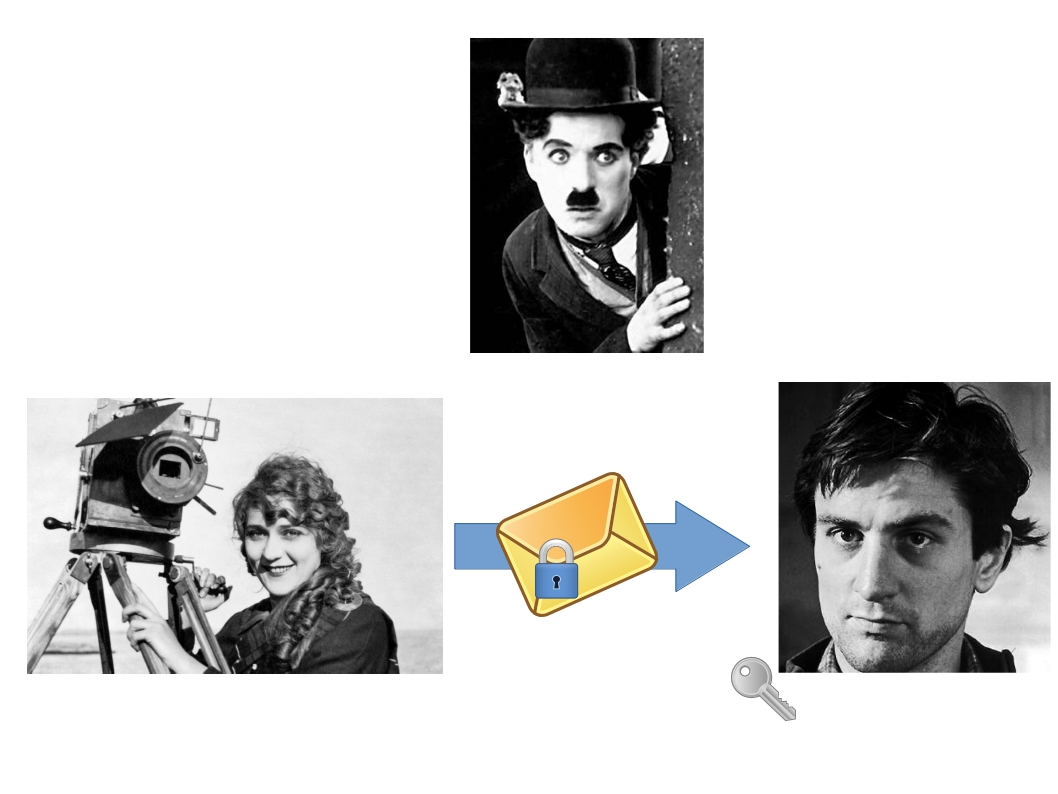
\includegraphics[scale=0.30]{Images/communication_Alice_Bob_chiffre.jpg} 
\end{center}
}
\only<3-3>{
\begin{center}
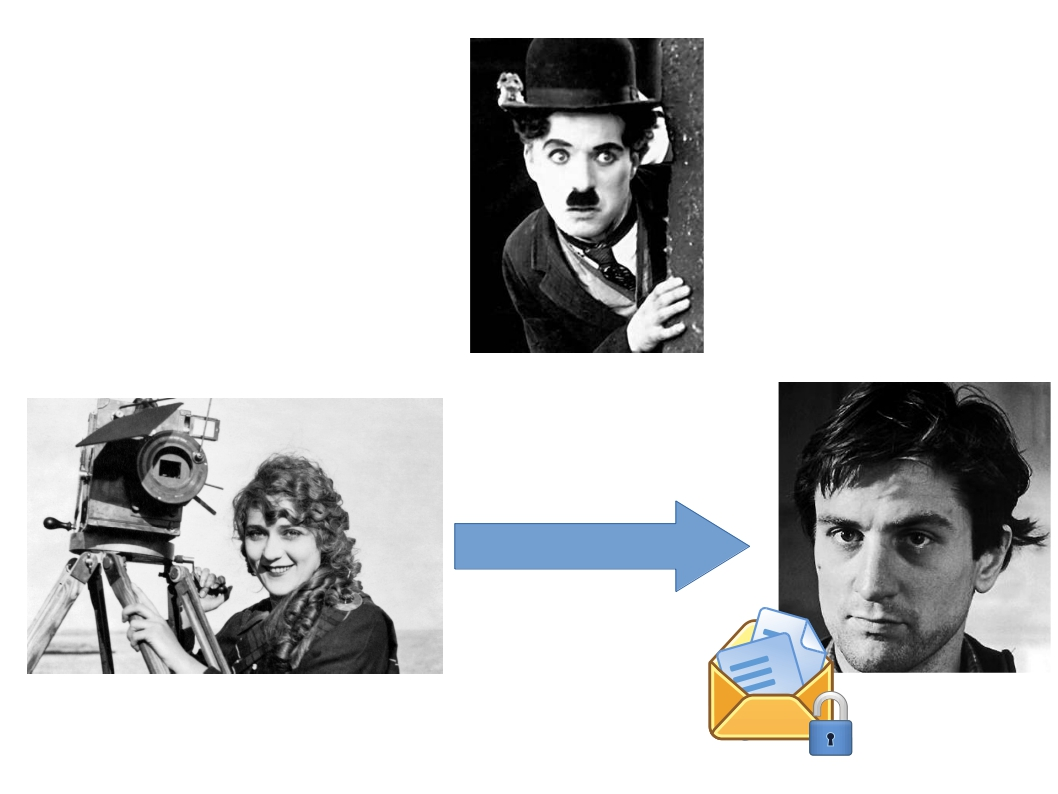
\includegraphics[scale=0.30]{Images/communication_Alice_Bob_dechiffre.jpg} 
\end{center}
}
%Dire que cette protection se fait a l aide d unn probleme mathematique juge  difficile
%parler de canaux non-sécurisés...
%\bluebox{Cryptography}
%{It is a way to communicate in a secured way on a channel that is not}

% parle de cryptographie symmétrique la clé de chiffrement et de déchiffrement sont identiques, et asymmétriques la clé de chiffrement et de déchiffrement sont différentes...
\end{frame}

